\documentclass{article}
\usepackage{geometry}[margin=0.25in]
\usepackage{amsmath}
\usepackage{amssymb}
\usepackage{graphicx}
\usepackage{hyperref}
\usepackage{array}
\usepackage{tocloft}
\usepackage{float}
\usepackage{empheq}
\usepackage{paracol}
\usepackage{enumitem}
\usepackage{multirow}
\usepackage[most]{tcolorbox}
\usepackage{titlesec}

\titleclass{\subsubsubsection}{straight}[\subsection]

\newcounter{subsubsubsection}[subsubsection]
\renewcommand\thesubsubsubsection{\thesubsubsection.\arabic{subsubsubsection}}
\renewcommand\theparagraph{\thesubsubsubsection.\arabic{paragraph}}
\titleformat{\subsubsubsection}
  {\normalfont\normalsize\bfseries}{\thesubsubsubsection}{1em}{}
\titlespacing*{\subsubsubsection}
{0pt}{3.25ex plus 1ex minus .2ex}{1.5ex plus .2ex}

\makeatletter
\renewcommand\paragraph{\@startsection{paragraph}{5}{\z@}%
  {3.25ex \@plus1ex \@minus.2ex}%
  {-1em}%
  {\normalfont\normalsize\bfseries}}
\renewcommand\subparagraph{\@startsection{subparagraph}{6}{\parindent}%
  {3.25ex \@plus1ex \@minus .2ex}%
  {-1em}%
  {\normalfont\normalsize\bfseries}}
\def\toclevel@subsubsubsection{4}
\def\toclevel@paragraph{5}
\def\l@subsubsubsection{\@dottedtocline{4}{7em}{4em}}
\def\l@paragraph{\@dottedtocline{5}{10em}{5em}}

\makeatother

\setcounter{secnumdepth}{4}
\setcounter{tocdepth}{5}

\renewcommand{\arraystretch}{1.5}
\hypersetup{
    colorlinks=true,
    linkcolor=black,
    filecolor=magenta,      
    urlcolor=black,
    pdfpagemode=FullScreen,
    pdfstartview=FitH,
}

\tcbset{colframe=black, colback=white, boxrule=1pt, breakable}

\begin{document}
\pagenumbering{roman}
\urlstyle{same}
%Title page

\begin{titlepage}
    \begin{center}
        \vspace*{1cm}
        \Huge
        3K04 Deliverable 1: Documentation
        \vspace{1cm}\\
        \huge
        Group 33
        \normalsize
        \vfill
        Last Updated: 2025-10-26
    \end{center}
 \end{titlepage}

%------------------------------------------------------------%

\newpage
\tableofcontents

%------------------------------------------------------------%

\newpage
\phantomsection
\listoffigures
\addcontentsline{toc}{section}{List of Figures}

\phantomsection
\listoftables
\addcontentsline{toc}{section}{List of Tables}

%------------------------------------------------------------%

\clearpage
\pagenumbering{arabic}
\newpage
\section{Group Members}
\begin{tabular}{|c|c|c|}
    \hline
    Name        & MacID         & Student Number    \\
    \hline
    Ryan Su     & sur21         & 400507973         \\
    \hline
    Cameron Lin & lin422        & 400535393         \\
    \hline
    Braden McEachern & mceacb1  & 400527617 \\
    \hline
    Damian Szydlowski & szydlowd & 400512629 \\
    \hline
    Menakan Thamilchelvan & thamilcm & 400510755\\ 
    \hline
\end{tabular}

\newpage
\section{Abbreviations}
\subsection{General Abbreviations}
\begin{enumerate}[label=]
    \item \textbf{BPM} - Beats Per Minute
    \item \textbf{CCS} - Cardiac Conduction System
    \item \textbf{DCM} - Device Controller-Monitor
    \item \textbf{GPIO} - General Purpose Input Output
    \item \textbf{GUI} - Graphical User Interface
    \item \textbf{PWM} - Pulse Width Modulation
\end{enumerate}

\subsection{Bradycardia Operating Abbreviations}
\begin{table}[H]
    \caption{Bradycardia Operating Abbreviations}
    \begin{tabular}{|m{2cm}|m{2cm}|m{2cm}|m{2cm}|m{3cm}|}
        \hline
        \textbf{Category} & \textbf{Chambers Paced} & \textbf{Chambers Sensed} & \textbf{Response to Sensing} & \textbf{Rate Modulation} \\
        \hline 
        Letters     & O-None & O-None & O-None & R-Rate Modulation\\
                    & A-Atrium & A-Atrium & T-Triggered & \\
                    & V-Ventricle & V-Ventricle & I-Inhibited & \\
                    & D-Dual & D-Dual & D-Tracked & \\
        \hline
    \end{tabular}
\end{table}
\newpage
\section{Part 1}

\subsection{Introduction}

It is hard to understate the importance of the human heart. The heart is the core part of the cardiovascular system; supplying nutrients and oxygen to all the cells
and removing carbon dioxide, especially to vital organs such as the brain, it is imperative for it to be working flawlessly and harmoniously at all times.
Unfortunately, however, cardiovascular diseases are a leading cause of death globally, many of which are caused from complications with 
abnormal heart rhythms. A pacemaker is an implantable device capable of sending timed electrical impulses causing contractions at 
appropriate intervals. Understanding the operation and design of this life saving device will aid in developing 
more efficient and reliable cardiac assistive technology. 

The purpose of this project is to design and implement a system that operates a cardiac pacemaker 
under specified modes. This project will be accomplished through an understanding of embedded systems and through engineering 
principles of software development. 

The scope of this deliverable is to design and implement the embedded pacemaker software, driver software and user interface for 
the DCM while updating and maintaining documentation. 



\subsection{Requirements}

\begin{itemize}
    \item Overall system requirements (summarized from provided specification documents). It can be informal or semi-formal.
    \item Mode-specific requirements: AOO, VOO, AAI, VVI.
\end{itemize}

\subsubsection{DCM Requirements}
The user shall be capable of the following:
\begin{itemize}
    \item Utilizing and managing windows for display of text and graphics.
    \item Processing user positioning and input buttons.
    \item Displaying all programmable parameters for review and modification.
    \item Visually indicating when telemetry is lost due to the device being out of range or noise.
    \item Vndicating when a different PACEMAKER device is approached than was previously interrogated
\end{itemize}

\newpage
\subsection{Design}
\label{dessec}
In this section, you want to expand on the design decisions based on the requirements. You should be specific about your system design and how the various components relate together.

\begin{itemize}
    \item System architecture (major subsystems, hardware hiding, pin mapping).
    \item Programmable parameters (rate limits, amplitudes, pulse widths, refractory periods, etc.).
    \item Hardware inputs and outputs (signals sensed, signals controlled).
    \item State machine design for each pacing mode (with diagrams if applicable). You can also use a tabular method.
    \item Simulink diagram
    \item Screenshots of your DCM, explaining its software structure
\end{itemize}

You should also be explicit on how your design decisions map directly to the requirements.

\newpage
\subsubsection{Simulink Design}

\subsubsubsection{Overall Design}

\begin{tcolorbox}
    \begin{figure}[H]
        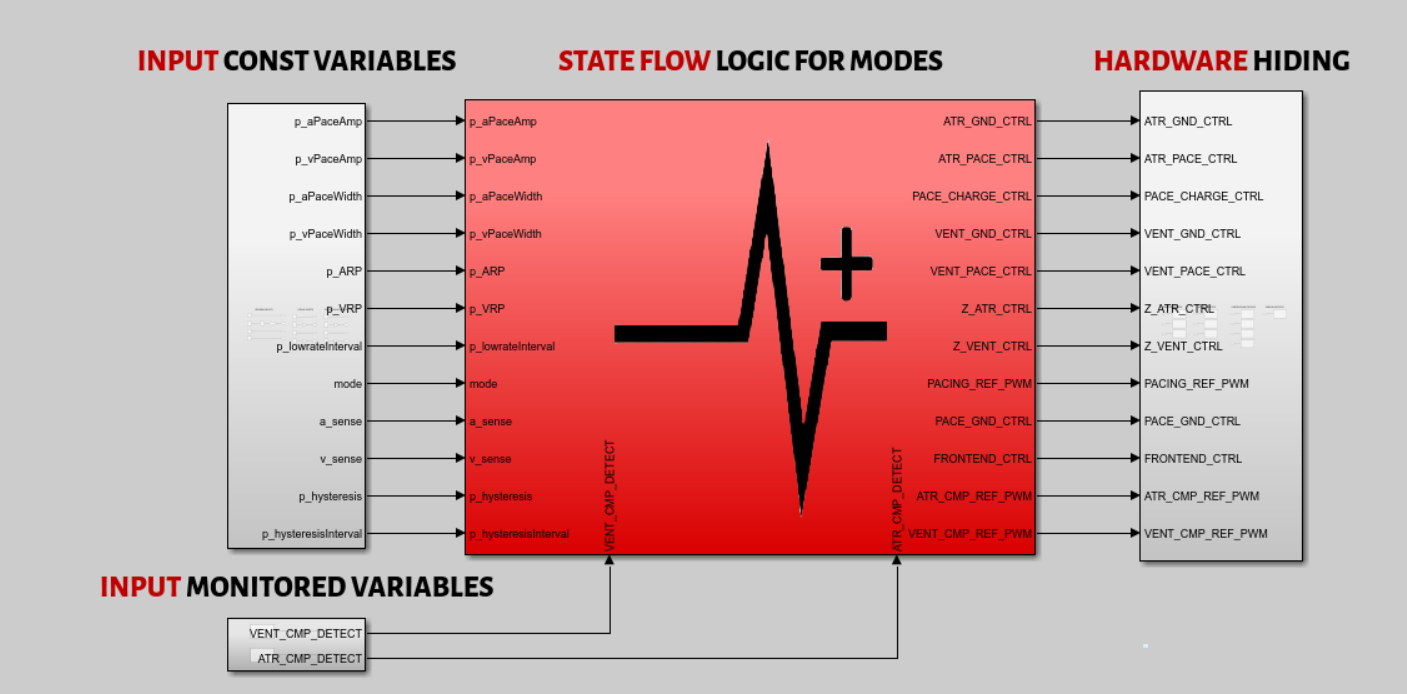
\includegraphics[width=\textwidth]{SimWholeView.png}
        \caption{Overall Simulink Mapping}
        \label{SimWholeView}
    \end{figure}
\end{tcolorbox}
The Pacemaker architecure can be split up into 4 main modules, input constant variables, 
input monitor variables, stateflow logic for modes, and hardware hiding. \hyperref[SimWholeView]{Figure 1} below shows the overarcing 
workflow of the system:

\newpage
\subsubsubsection{Input Constant Variables}

\begin{tcolorbox}
    \begin{figure}[H]
        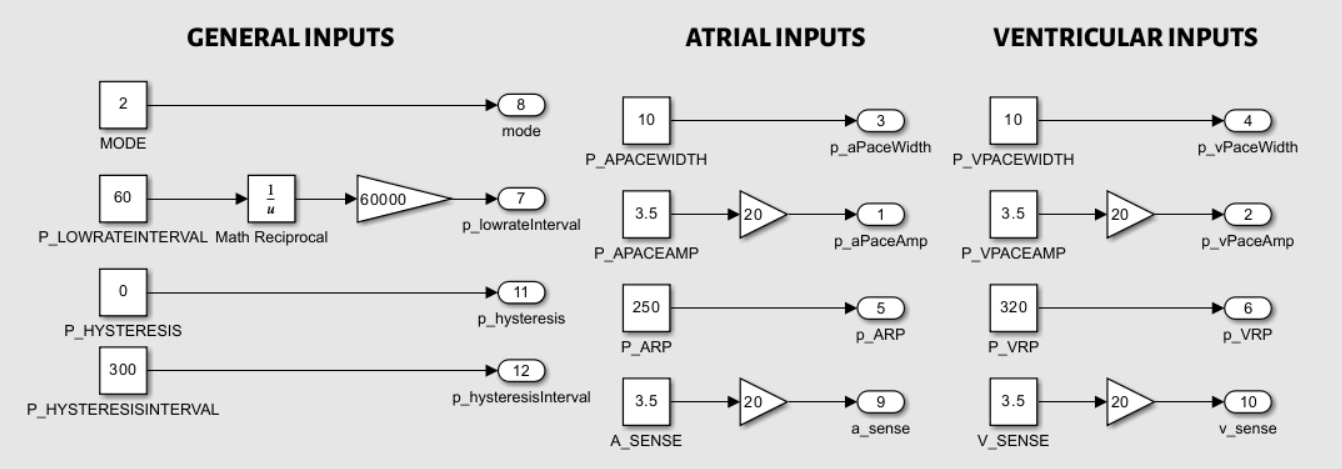
\includegraphics[width=\textwidth]{ConstIn.png}
        \caption{Constant Input Variables}
        \label{ConstIn}
    \end{figure}
\end{tcolorbox}
In the above image, \hyperref[ConstIn]{Figure 2}, we find changeable variables 
relating to pacemaker operation. For general inputs, the changeable variables are:

\begin{itemize}
    \item \textbf{Mode} - Refers to bradycardia operating modes, e.g AOO, VOO, AAI and VVI.
    \item \textbf{Low Rate Interval} - The number of generated pace pulses per minute, converted from a millisecond time period. 
    \item \textbf{Hysteresis Pace} - When enabled, 1, a longer period is waited before pacing after sensing an event to prevent unwanted pacing pulses from ringing from an event. 
    \item \textbf{Hysteresis Interval} - Specifies the time interval waited in the hysteresis mode in milliseconds.
\end{itemize}
The modfiable atrial variables are:

\begin{itemize}
    \item \textbf{Pace Pulse Width} - Changes the width, length of time, of the pace pulse.
    \item \textbf{Pace Pulse Amplitude} - Changes the amplitude, voltage, of the pace pulse.
    \item \textbf{ARP (Atrial Refactory Period)} - The programmed time interval following an atrial event during which time atrial
            events shall not inhibit nor trigger pacing
    \item \textbf{Sense (Sensitivity)} - Determines the minimum value an atrial signal must be to be considered by the pacemaker. 
\end{itemize}
The modifiable ventricular variables are:

\begin{itemize}
    \item \textbf{Pace Pulse Width} - Changes the width, length of time, of the pace pulse.
    \item \textbf{Pace Pulse Amplitude} - Changes the amplitude, voltage, of the pace pulse.
    \item \textbf{VRP (Ventricle Refactory Period)} - The programmed time interval following an ventricle event during which time atrial
            events shall not inhibit nor trigger pacing.
    \item \textbf{Sense (Sensitivity)} - Determines the minimum value a ventricle signal must be to be considered by the pacemaker.
\end{itemize}

\newpage
\subsubsubsection{Monitored Input Variables}

\begin{tcolorbox}
    \begin{figure}[H]
        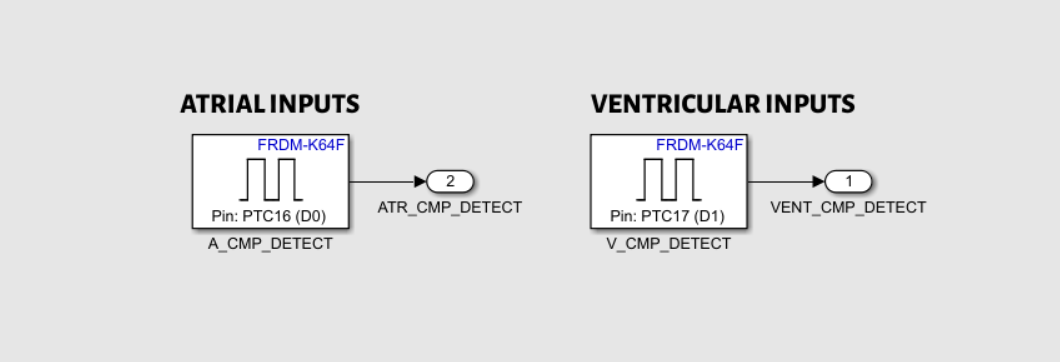
\includegraphics[width=\textwidth]{InMon.png}
        \caption{Monitored Input Variables}
        \label{InMon}
    \end{figure}
\end{tcolorbox}
The monitored input variables can be seen in the above \hyperref[InMon]{Figure 3}. These are the atrial and ventricle detection 
variables. The pulses are sensed with through GPIO pins connecting to a board simulating heart conditions. 

\newpage
\subsubsubsection{Stateflow Modules}
\begin{tcolorbox}
    \begin{figure}[H]
        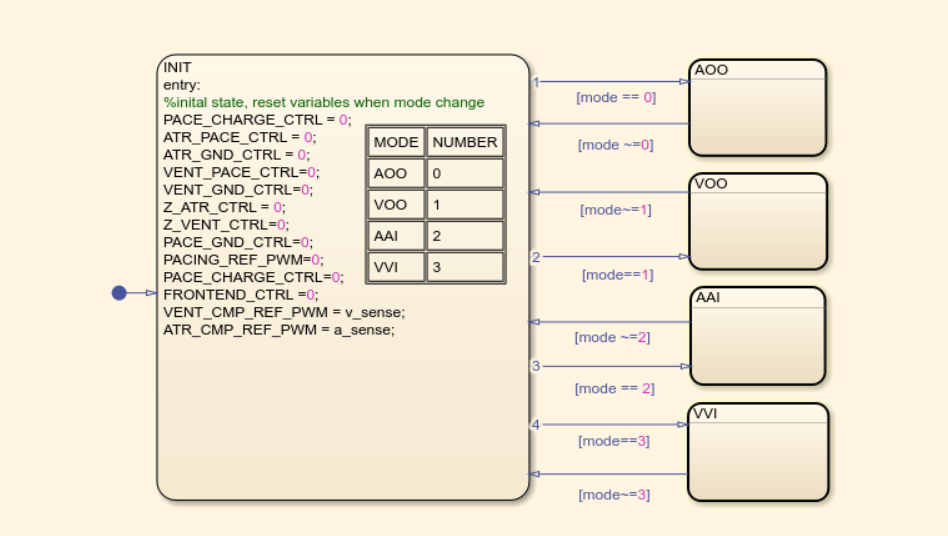
\includegraphics[width=\textwidth]{StateMod.png}
        \caption{Stateflow Modules}
        \label{StateMod}
    \end{figure}
\end{tcolorbox}
The stateflow diagram in Simulink is shown above. It shows the transition between each mode given the mode input shown in 
\hyperref[ConstIn]{Figure 2}. When switching between modes, a core state is returned to that resets variables to their nominal values. 

\newpage
\subsubsubsection{AOO Stateflow Model}
\begin{tcolorbox}
    \begin{figure}[H]
        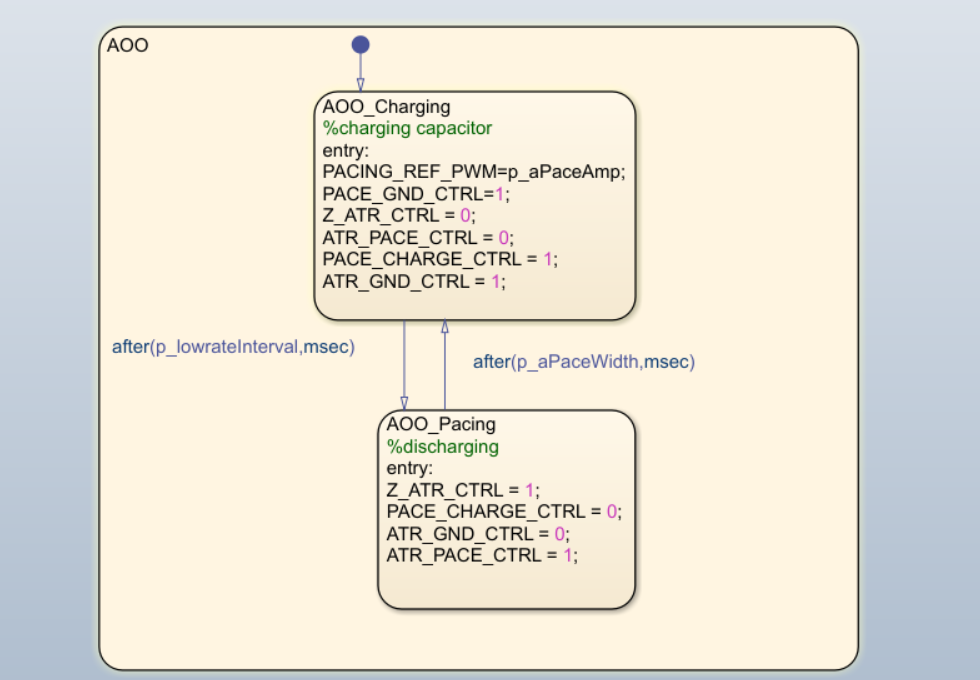
\includegraphics[width=\textwidth]{AOO.png}
        \caption{AOO Stateflow Model}
        \label{AOOSF}
    \end{figure}
\end{tcolorbox}
The above stateflow, \hyperref[AOOSF]{Figure 5}, shows the stateflow for the AOO mode. It sets values 
controlling discharge and charging of the capacitor to specified nominal values.

\newpage
\subsubsubsection{VOO Stateflow Model}
\begin{tcolorbox}
    \begin{figure}[H]
        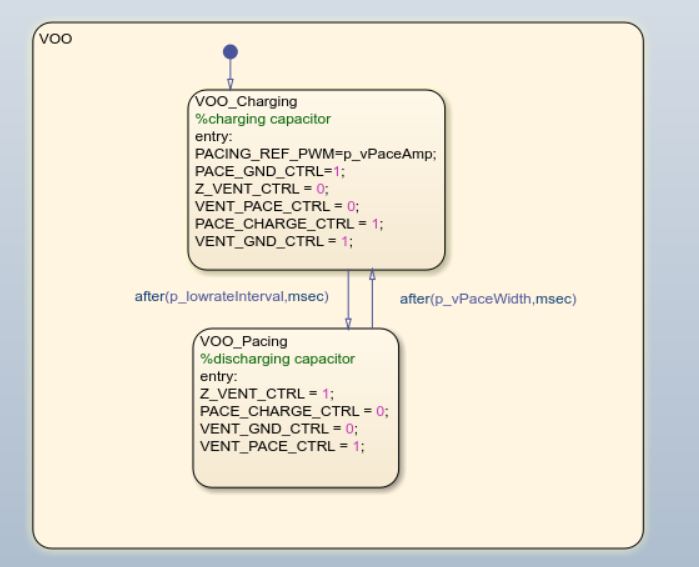
\includegraphics[width=\textwidth]{VOO.png}
        \caption{VOO Stateflow Model}
        \label{VOOSF}
    \end{figure}
\end{tcolorbox}
Similar to the AOO stateflow, the above figure, \hyperref[VOOSF]{Figure 6}, shows the states of 
charging and discharging of the capacitor using specified nominal values. 

\newpage
\subsubsubsection{VII Stateflow Model}
\begin{tcolorbox}
    \begin{figure}[H]
        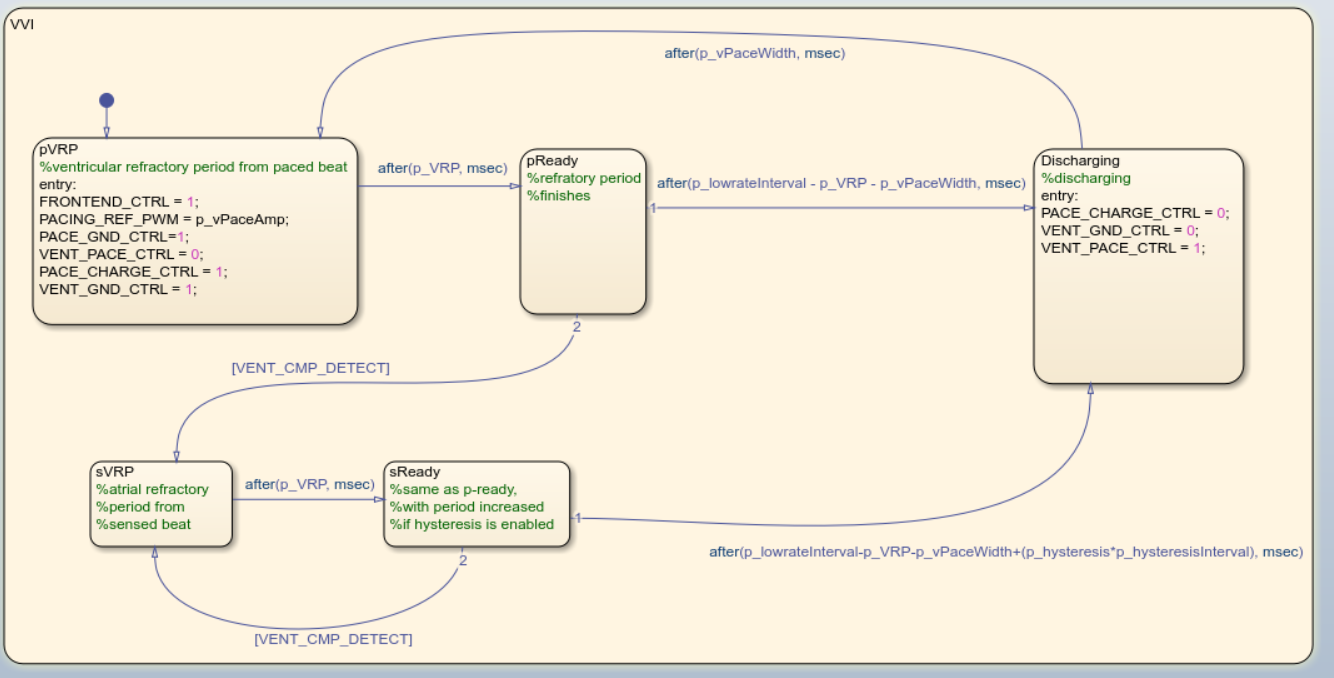
\includegraphics[width=\textwidth]{VVI.png}
        \caption{VVI Stateflow Model}
        \label{VVISF}
    \end{figure}
\end{tcolorbox}
The above stateflow, \hyperref[VVISF]{Figure 7} shows the FSM for the VVI model. The initial state, pVRP, is the state 
that occurs right after the pacemaker delivers a ventricle pacing pulse. A refactory period occurs during this time, where the 
pacemaker ignores sensor inputs to prevent sensing of its own produced pulse or electrical ringing. After a certain amount of time,
the pReady state is transitioned to where sensor inputs are allowed. This allows for the pacemaker to detect natural heart rhythms
and correct heart rhythms accordingly, or solely deliver pacing pulses. The last state before going to the initial state is the 
discharging state where the pacing pulse is produced. 

\newpage
\subsubsubsection{AAI Stateflow Model}
\begin{tcolorbox}
    \begin{figure}[H]
        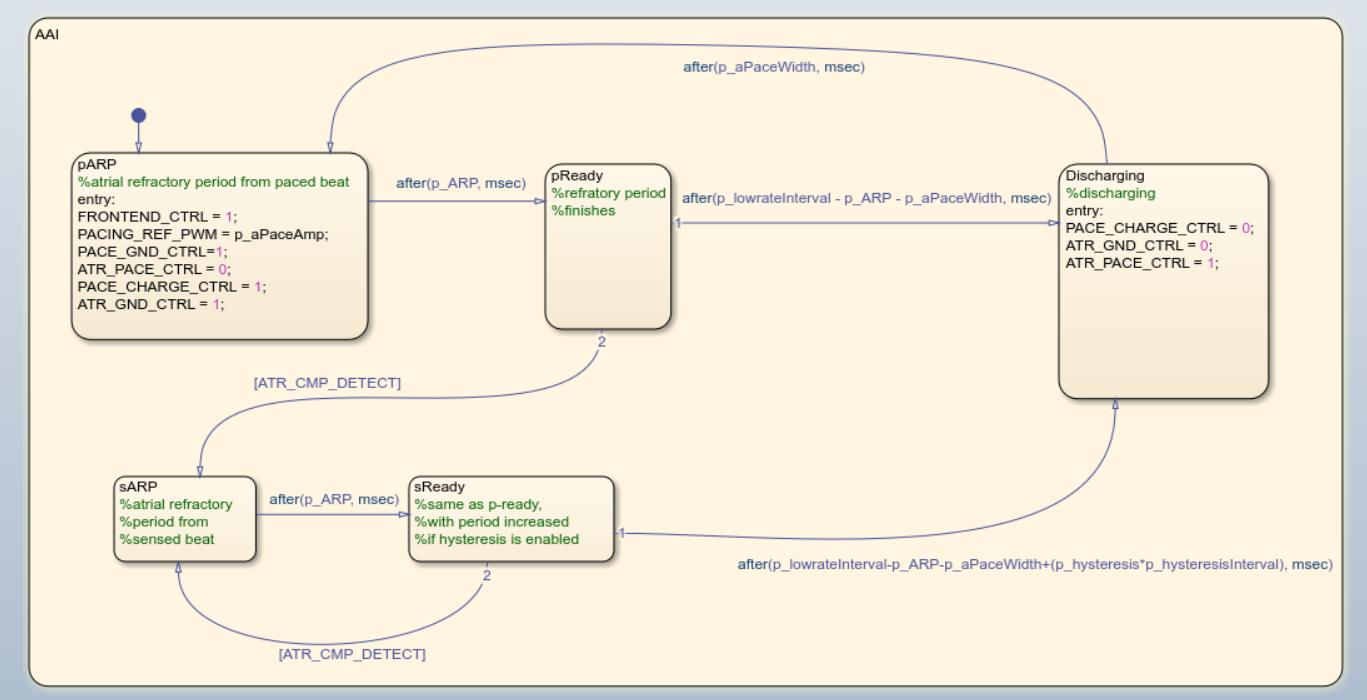
\includegraphics[width=\textwidth]{AAI.png}
        \caption{AAI Stateflow Model}
        \label{AAISF}
    \end{figure}
\end{tcolorbox}
The above stateflow, \hyperref[AAISF]{Figure 8} shows the process for the AAI mode. The initial state, pARP, is 
the state occurs right after the pacemaker delivers an atrial pacing pulse. During this time, the pacemaker ignores 
sensing events to prevent it from sensing its own delivered pulse. The next state is transitioned to after 
a set time period, the refactory period, if no natural heartbeat is detected after a certain time inverval, the 
discharging state is then transitioned to. However, if a natural heartbeat is detected, another refactory period occurs 
to prevent the pacemaker from sensing ringing. This state then transitions to the discharging state once an appropriate time 
has passed. 

\newpage
\subsubsubsection{Hardware Hiding}

\begin{tcolorbox}
    \begin{figure}[H]
        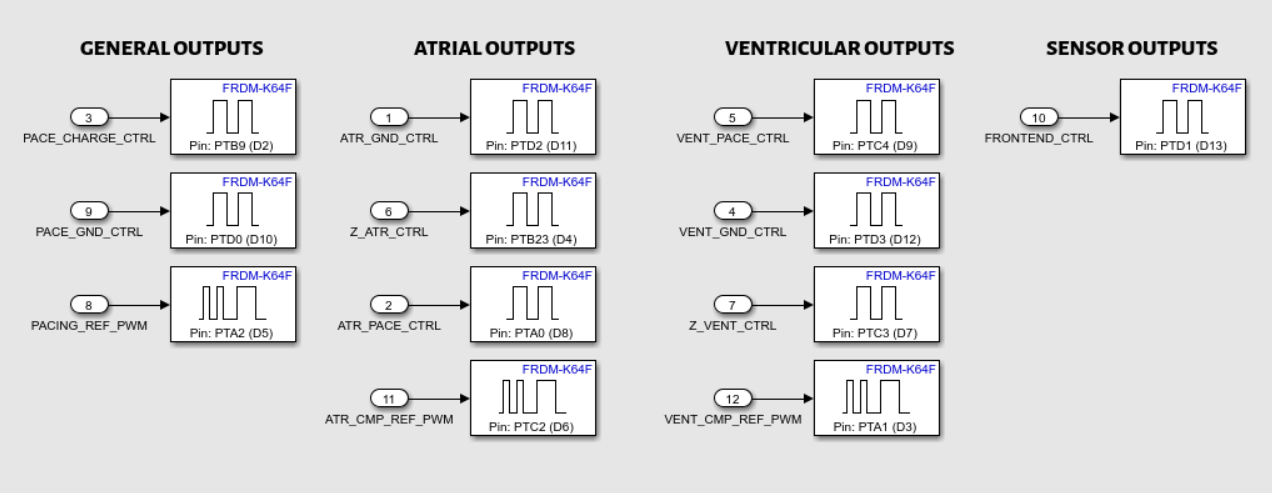
\includegraphics[width=\textwidth]{HardwareHiding.png}
        \caption{Hardware Hiding of Model}
        \label{HardHide}
    \end{figure}
\end{tcolorbox}

The above image, \hyperref[HardHide]{Figure 9} shows abstraction of the GPIO pin functions. 
It connects logical output signals to the pins on the FRDM-K64F. This allows for better readability,
thus making the code easier to maintain, debug and safer. 

\newpage
\subsubsection{DCM Design}

\newpage
\section{Part 2}

\subsection{Requirements Potential Changes}
Identify which requirements may evolve in the next deliverable (e.g., adding more modes, communication, new parameters).

\subsection{Design Decision Potential Changes}
List design choices that may need revisiting (e.g., choice of libraries, interface design, architecture).

\newpage
\subsection{Module Description}

Although breifly highlighted in the \hyperref[dessec]{design section} of this documentation. This section will go 
into more detail about the purpose of each module, key functionality, variables, and how each module interacts with 
one another. 

As shown in \hyperref[SimWholeView]{Figure 1}, there are 3 primary modules operating the pacemaker; \textbf{input constant variables, 
stateflow logic for modes, and hardware hiding.}

\subsubsection{Input Constant Variables Module}
This module is highlighted in the \hyperref[dessec]{design section}. It goes through all the state variables that 
are changeable parameters of the pacemaker. These inputs include general inputs such as the pacing mode, low rate interval, and hysteresis settings, as well 
as parameters for atrial and ventricle pacing. These parameters are then used in the stateflow logic module to 
complete pacing to user specifications.

\subsubsection{Stateflow Logic}
This module has many submodules which are also covered in the \hyperref[dessec]{design section}. The overall state machine controlling 
mode selection and reseting of variables to prevent unwanted pacing behaviour is shown in \hyperref[StateMod]{Figure 4}. This module 
converts input parameters into raw data that can be further converted to electrical signals. This module recieves data 
from the input constant variables module as well as from the monitored input variables. This module then feeds into 
hardware hiding. 

\subsubsection{Hardware Hiding}
Hardware hiding is also briefly covered in the \hyperref[dessec]{design section}. The purpose of this module is 
to convert the signals from the stateflow logic module into outputted electrical signals through pins. As shown in 
\hyperref[HardHide]{Figure 9}, pins are mapped to certain electrical signals such as atrial outputs, ventrical outputs, 
front end signals, and general pin configurations such as grounding pins. This is designed to ensure coding and modules 
are easier to debug with higher level identification and function of each GPIO. 

\newpage
\subsection{Testing}

\subsubsection{SimuLink Mode Testing}

\subsubsubsection{Testing of AOO}

\begin{enumerate}[label=]
   \item \textbf{Purpose:} The purpose of this test is to test basic AOO functionality.
   \item \textbf{Input Conditions:} General inputs of mode = 0, AOO, and hysteresis = 0, off, and standard 
   atrial inputs. 
   \item \textbf{Expected Output:} Consistent, evenly spaced pulses in the output with disregard for natural heart beats.
   \item \textbf{Actual Output:} Output of testing is exactly that of expected, as shown below in \hyperref[AOOtest]{Figure 10}.
   \item \textbf{Result:} Pass
\end{enumerate}

\begin{tcolorbox}
    \begin{figure}[H]        
        \label{AOOtest}
        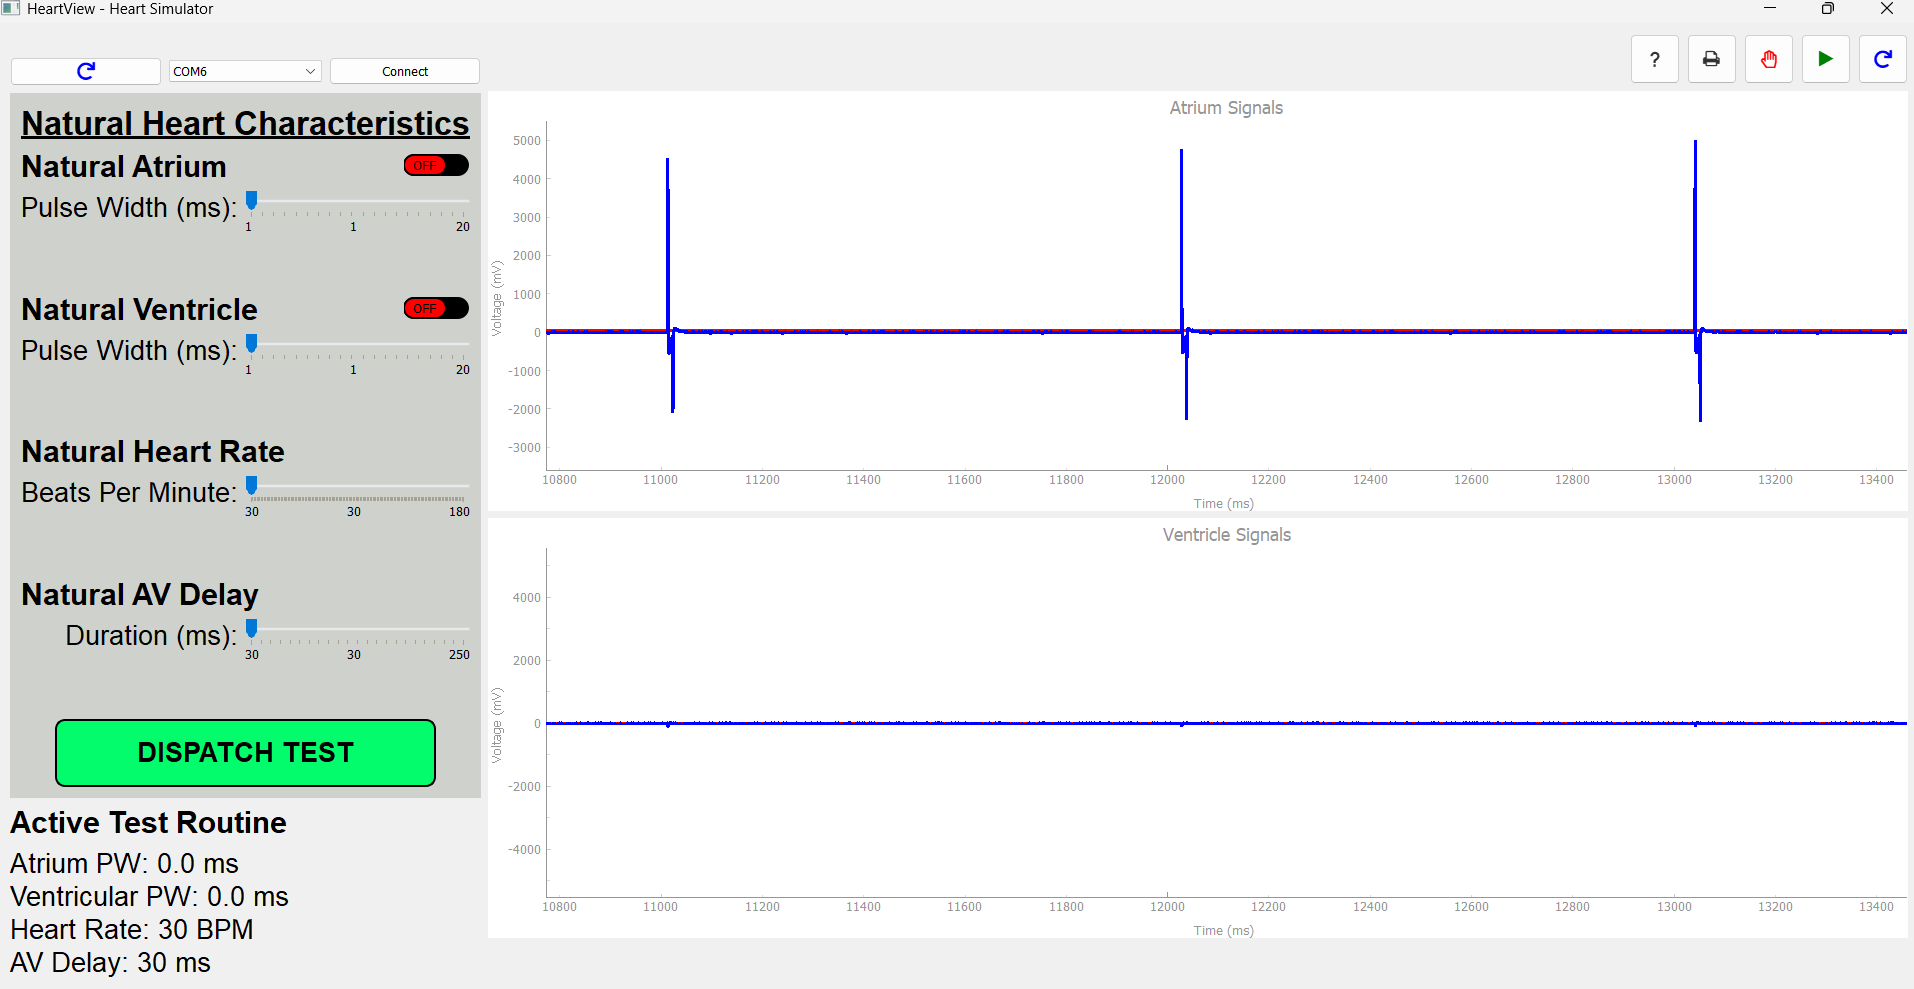
\includegraphics[width=\textwidth]{AOOtest1.png}
        \caption{AOO Test}
    \end{figure}
\end{tcolorbox}

\newpage
\hyperref[AOOpulse]{Figure 11} below shows a zoomed in view of one of the pulses in the AOO test above, \hyperref[AOOtest]{Figure 10}. 

\begin{tcolorbox}
    \begin{figure}[H]
        \label{AOOpulse}
        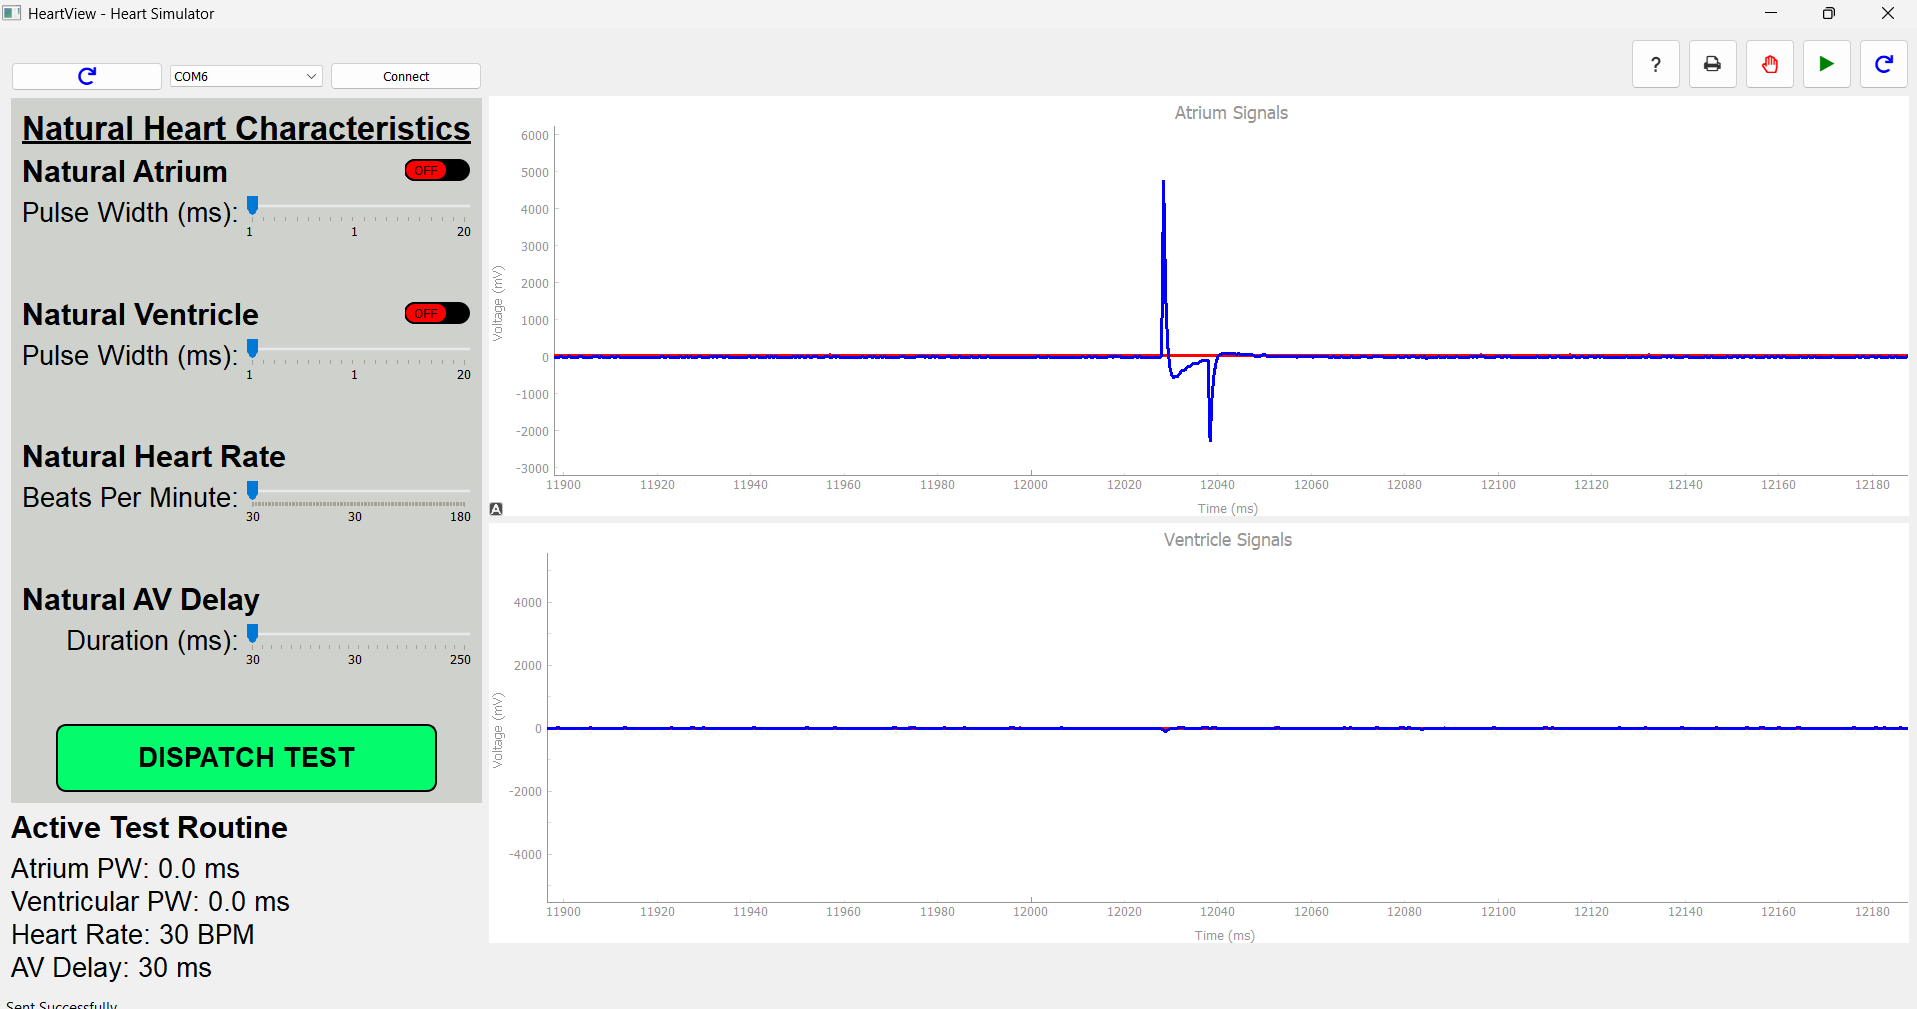
\includegraphics[width=\textwidth]{AOOPulseClose.png}
        \caption{Close-up of AOO Pulse}
    \end{figure}
\end{tcolorbox}

\newpage
\subsubsubsection{Testing of VOO}

\begin{enumerate}[label=]
   \item \textbf{Purpose:} The purpose of this test is to test basic VOO functionality.
   \item \textbf{Input Conditions:} General inputs of mode = 1, VOO, and hysteresis = 0, off, and standard 
   ventricle inputs. 
   \item \textbf{Expected Output:} Consistent, evenly spaced pulses in the output with disregard for natural heart beats.
   \item \textbf{Actual Output:} Output of testing is exactly that of expected, as shown below in \hyperref[VOOtest]{Figure 12}.
   \item \textbf{Result:} Pass
\end{enumerate}

\begin{tcolorbox}
    \begin{figure}[H]
        \label{VOOtest}
        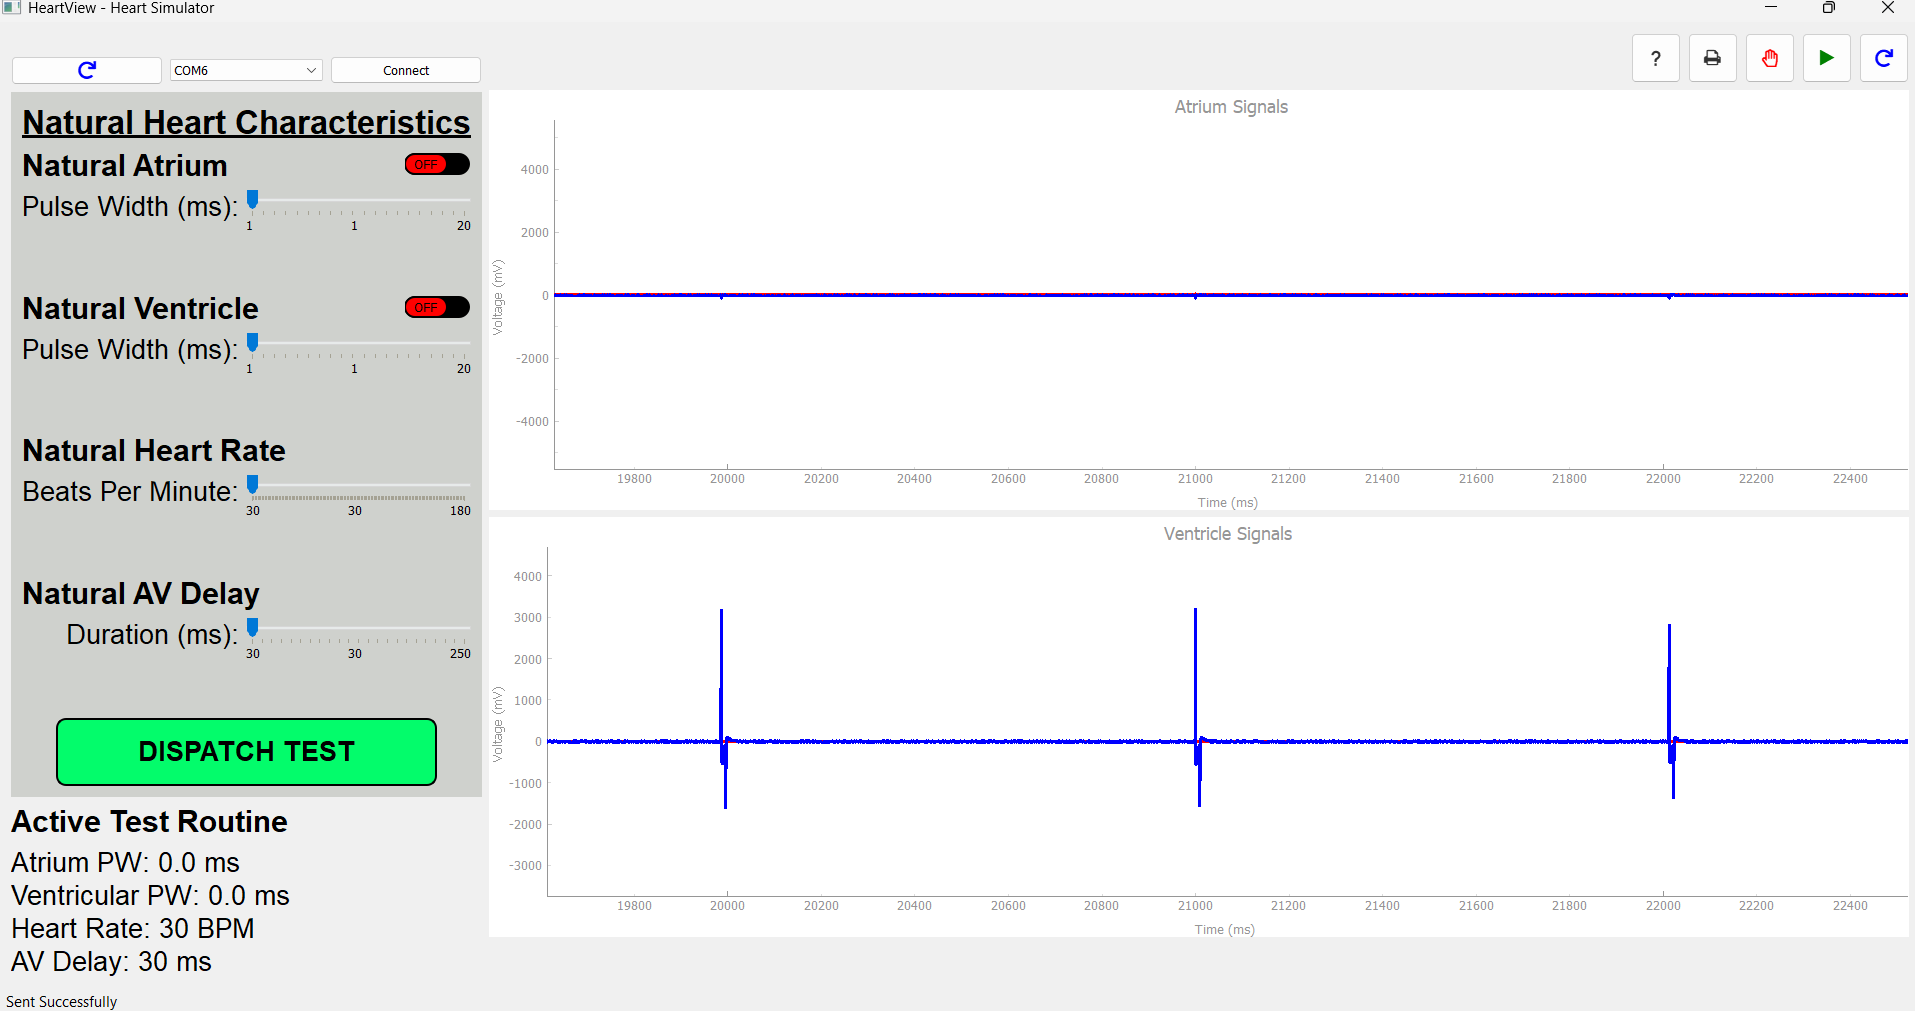
\includegraphics[width=\textwidth]{VOOtest.png}
        \caption{VOO Test}
    \end{figure}
\end{tcolorbox}

\newpage
\hyperref[VOOpulseclose]{Figure 13} below shows a zoomed in view of one of the pulses in the VOO test above, \hyperref[VOOtest]{Figure 12}

\begin{tcolorbox}
    \begin{figure}[H]
        \label{VOOpulseclose}
        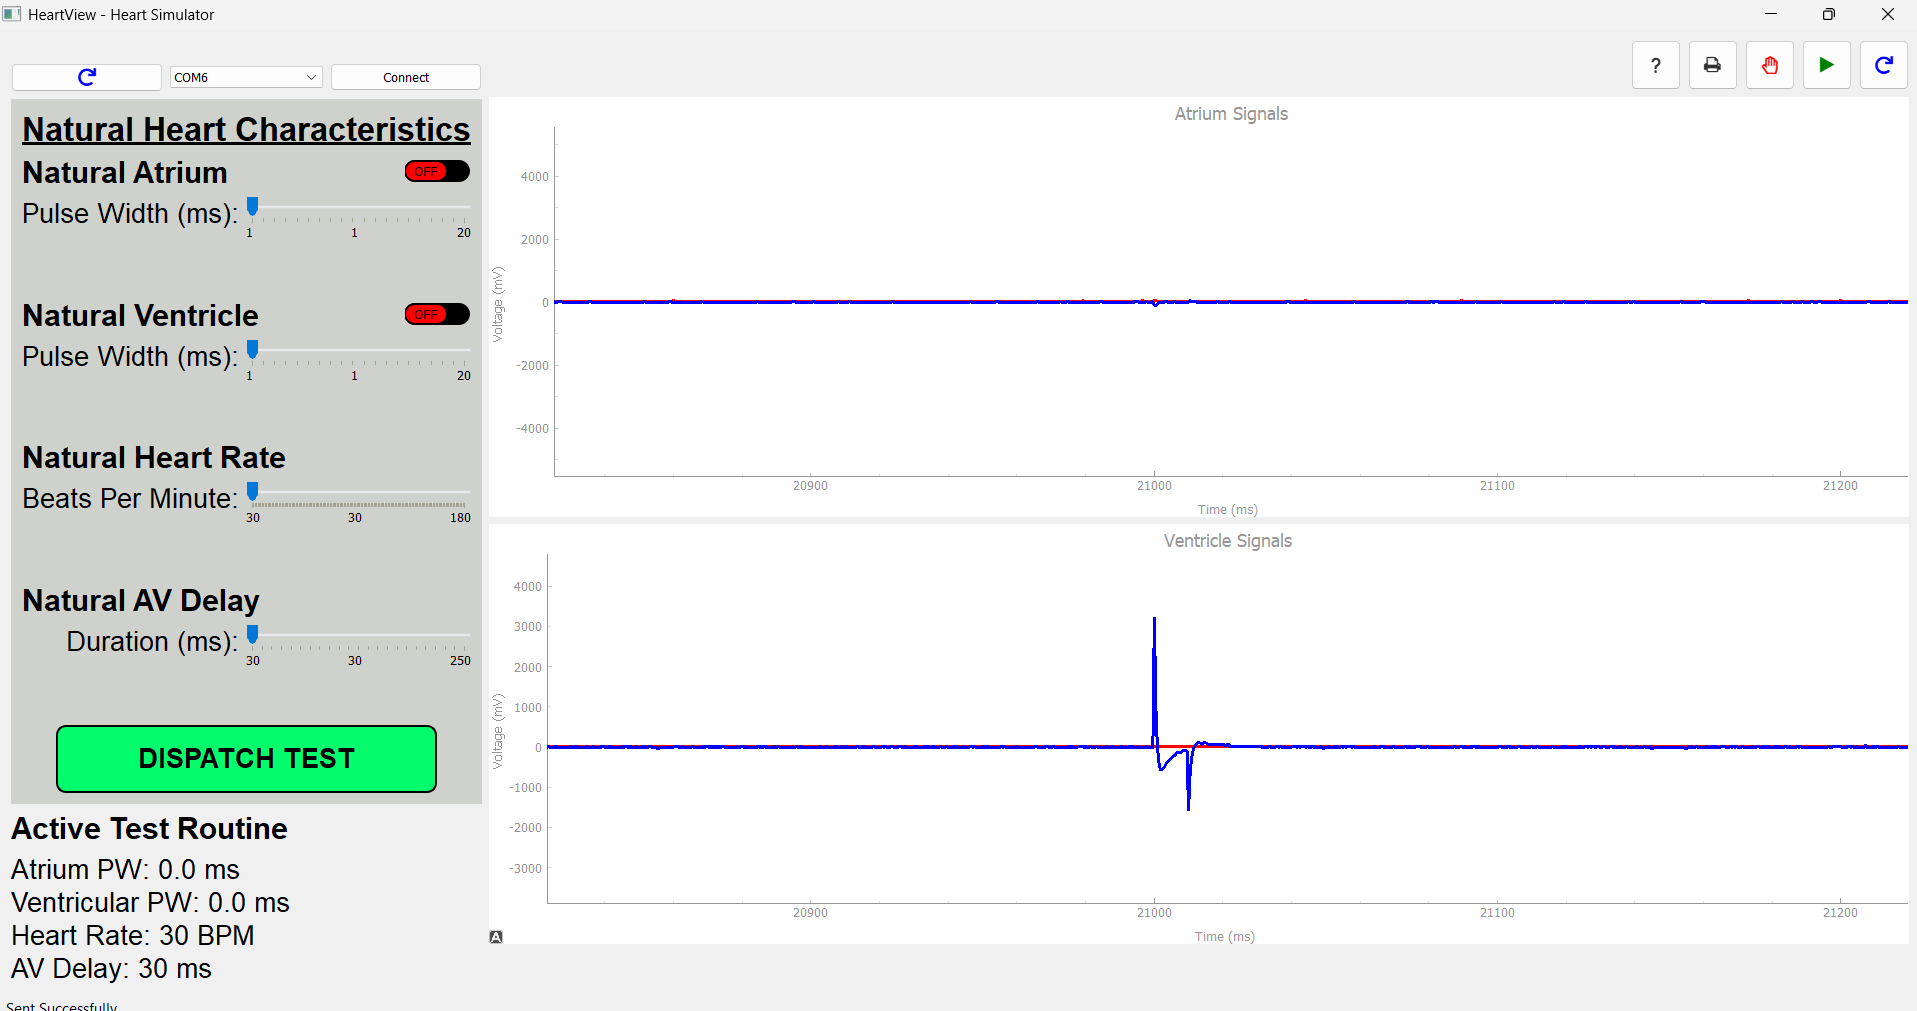
\includegraphics[width=\textwidth]{VOOpulseclose.png}
        \caption{Close-up of VOO Pulse}
    \end{figure}
\end{tcolorbox}

\newpage
\subsubsubsection{Testing of AAI}

\paragraph{No Natural Heart Rate}

\begin{enumerate}[label=]
   \item \textbf{Purpose:} The purpose of this test is to test basic AAI functionality with no natural heart rhythms.
   \item \textbf{Input Conditions:} General inputs of mode = 2, AAI, and hysteresis = 0, off, and standard 
   artial inputs. 
   \item \textbf{Expected Output:} Consistent, evenly spaced pulses in the output.
   \item \textbf{Actual Output:} Output of testing is exactly that of expected, as shown below in \hyperref[AAItestnohr]{Figure 13}.
   \item \textbf{Result:} Pass
\end{enumerate}

\begin{tcolorbox}
    \begin{figure}[H]
        \label{AAItestnohr}
        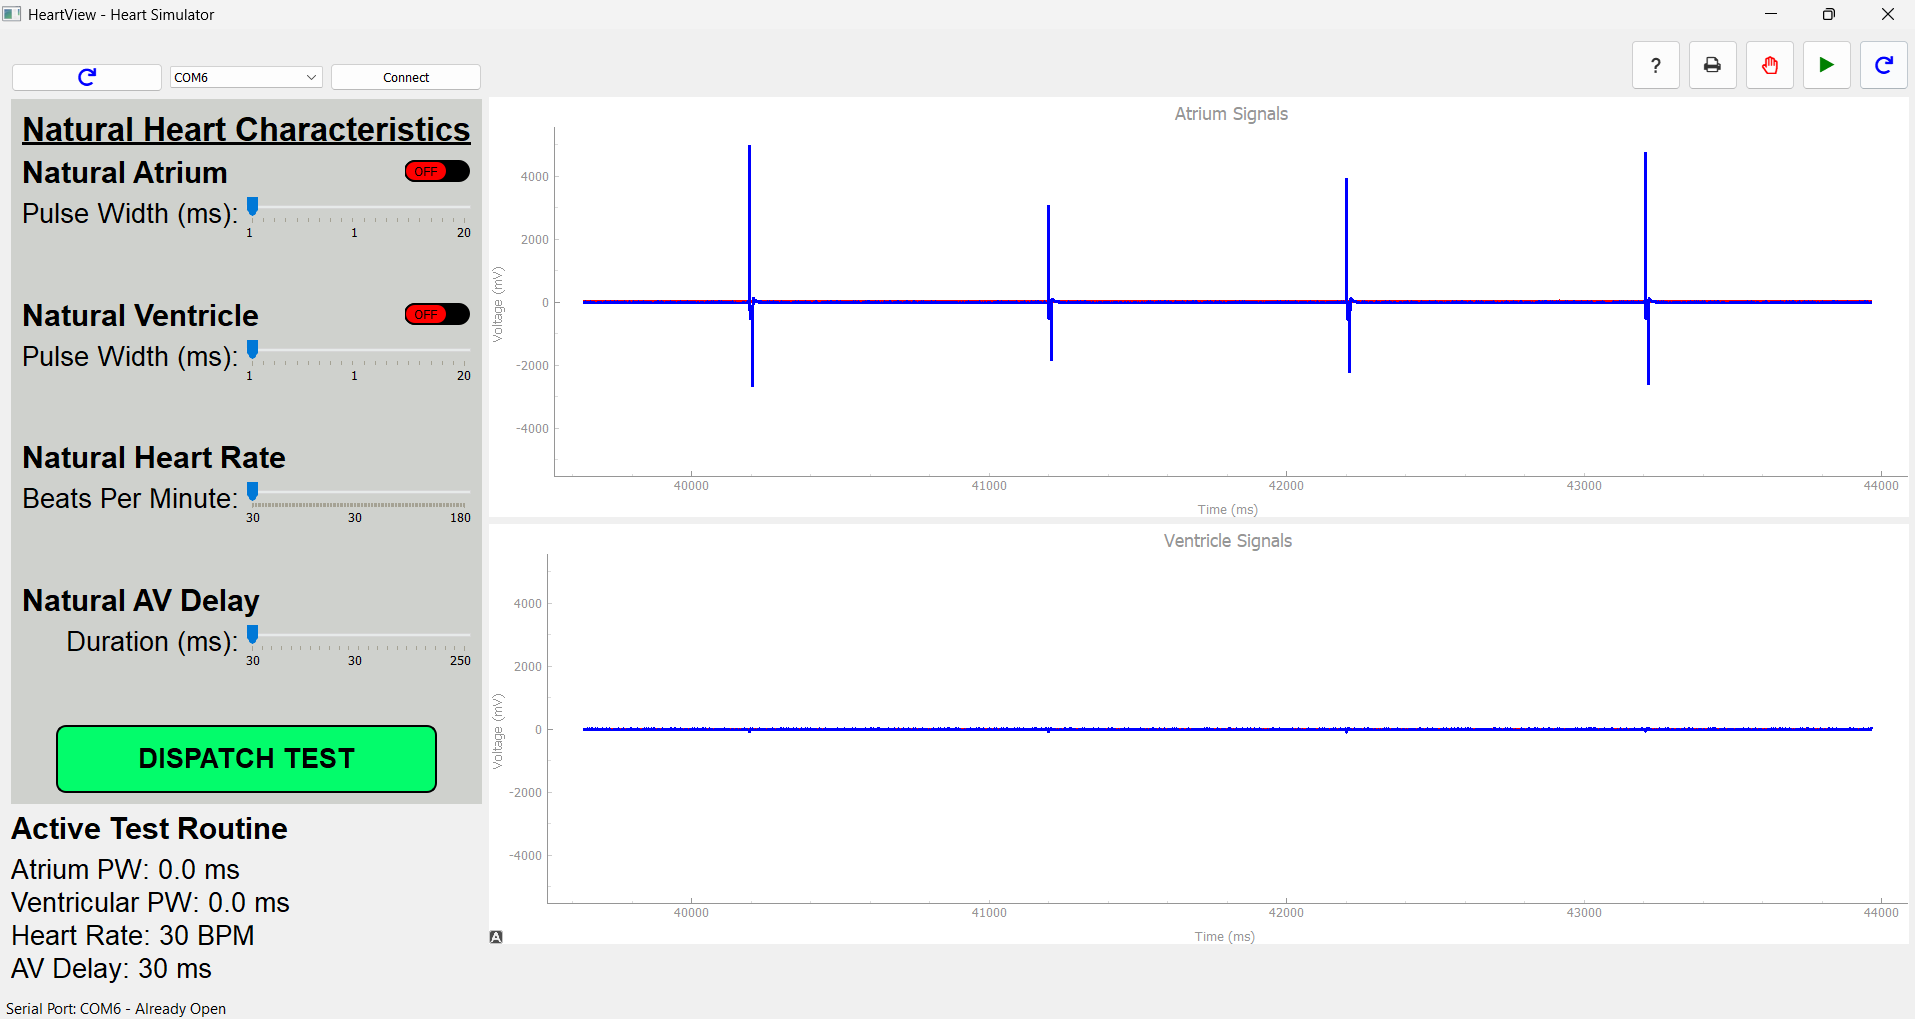
\includegraphics[width=\textwidth]{AAItestnohr.png}
        \caption{AAI Test No Heart Rate}
    \end{figure}
\end{tcolorbox}

\newpage
\paragraph{Natural Heart Rate of 45 BPM}

\begin{enumerate}[label=]
   \item \textbf{Purpose:} The purpose of this test is to test basic AAI functionality at a low heart rate.
   \item \textbf{Input Conditions:} General inputs of mode = 2, AAI, and hysteresis = 0, off, standard 
   artial inputs, and monitored atrial pulses at 45 BPM.
   \item \textbf{Expected Output:} The pacemaker should pulse after the refactory period expires. An output of blue pulses right before the natural 
   red pulses is expected.
   \item \textbf{Actual Output:} Output of testing is exactly that of expected, as shown below in \hyperref[AAItest45]{Figure 15}.
   \item \textbf{Result:} Pass
\end{enumerate}


\begin{tcolorbox}
    \begin{figure}[H]\label{AAItest45}
        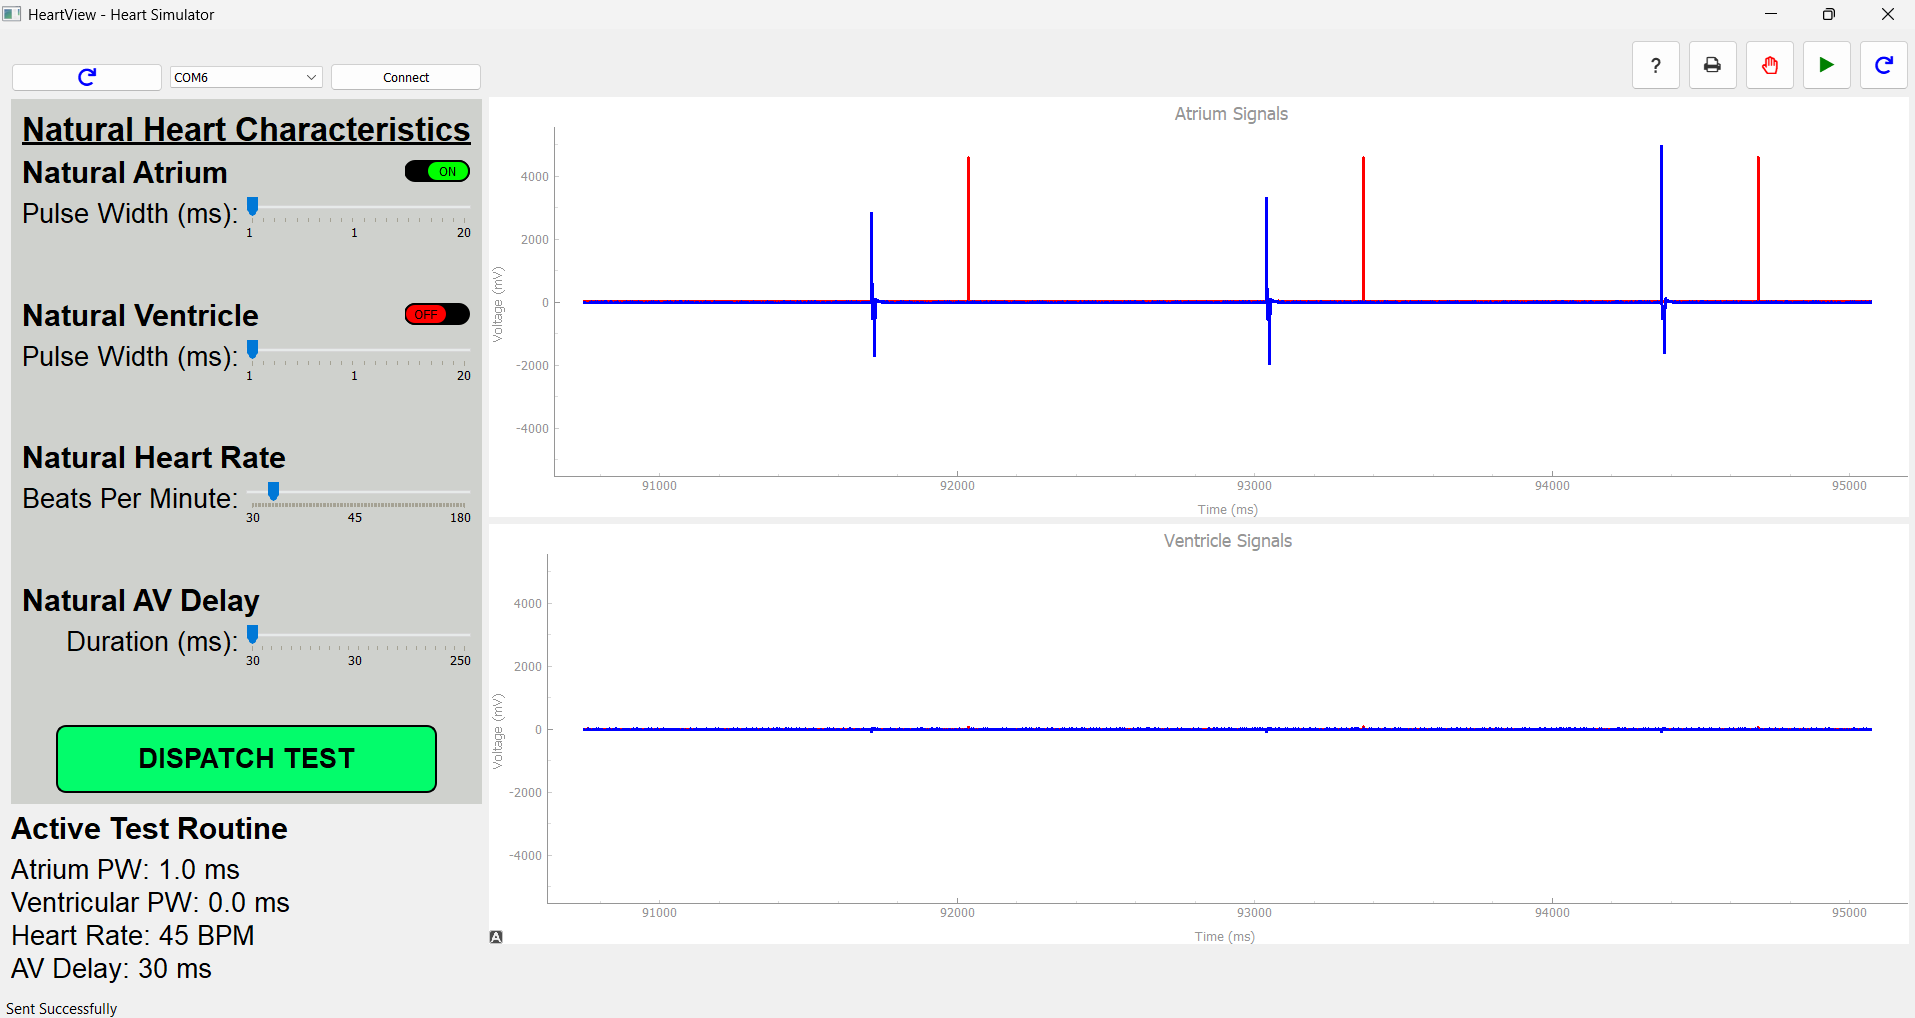
\includegraphics[width=\textwidth]{AAItest45.png}
        \caption{AAI Test 45 BPM}      
    \end{figure}
\end{tcolorbox}

\newpage
\paragraph{Natural Heart Rate of 75 BPM}

\begin{enumerate}[label=]
   \item \textbf{Purpose:} The purpose of this test is to test basic AAI functionality at a nominal heart rate.
   \item \textbf{Input Conditions:} General inputs of mode = 2, AAI, and hysteresis = 0, off, standard 
   artial inputs, and monitored atrial pulses at 75 BPM.
   \item \textbf{Expected Output:} As a nominal heart reate is being inputted, the pacemaker should not be delivering pacing pulses 
   as the simulated heart rate is nominal and healthy.
   \item \textbf{Actual Output:} Output of testing is exactly that of expected, as shown below in \hyperref[AAItest75]{Figure 16}.
   \item \textbf{Result:} Pass
\end{enumerate}

\begin{tcolorbox}
    \begin{figure}[H]\label{AAItest75}
        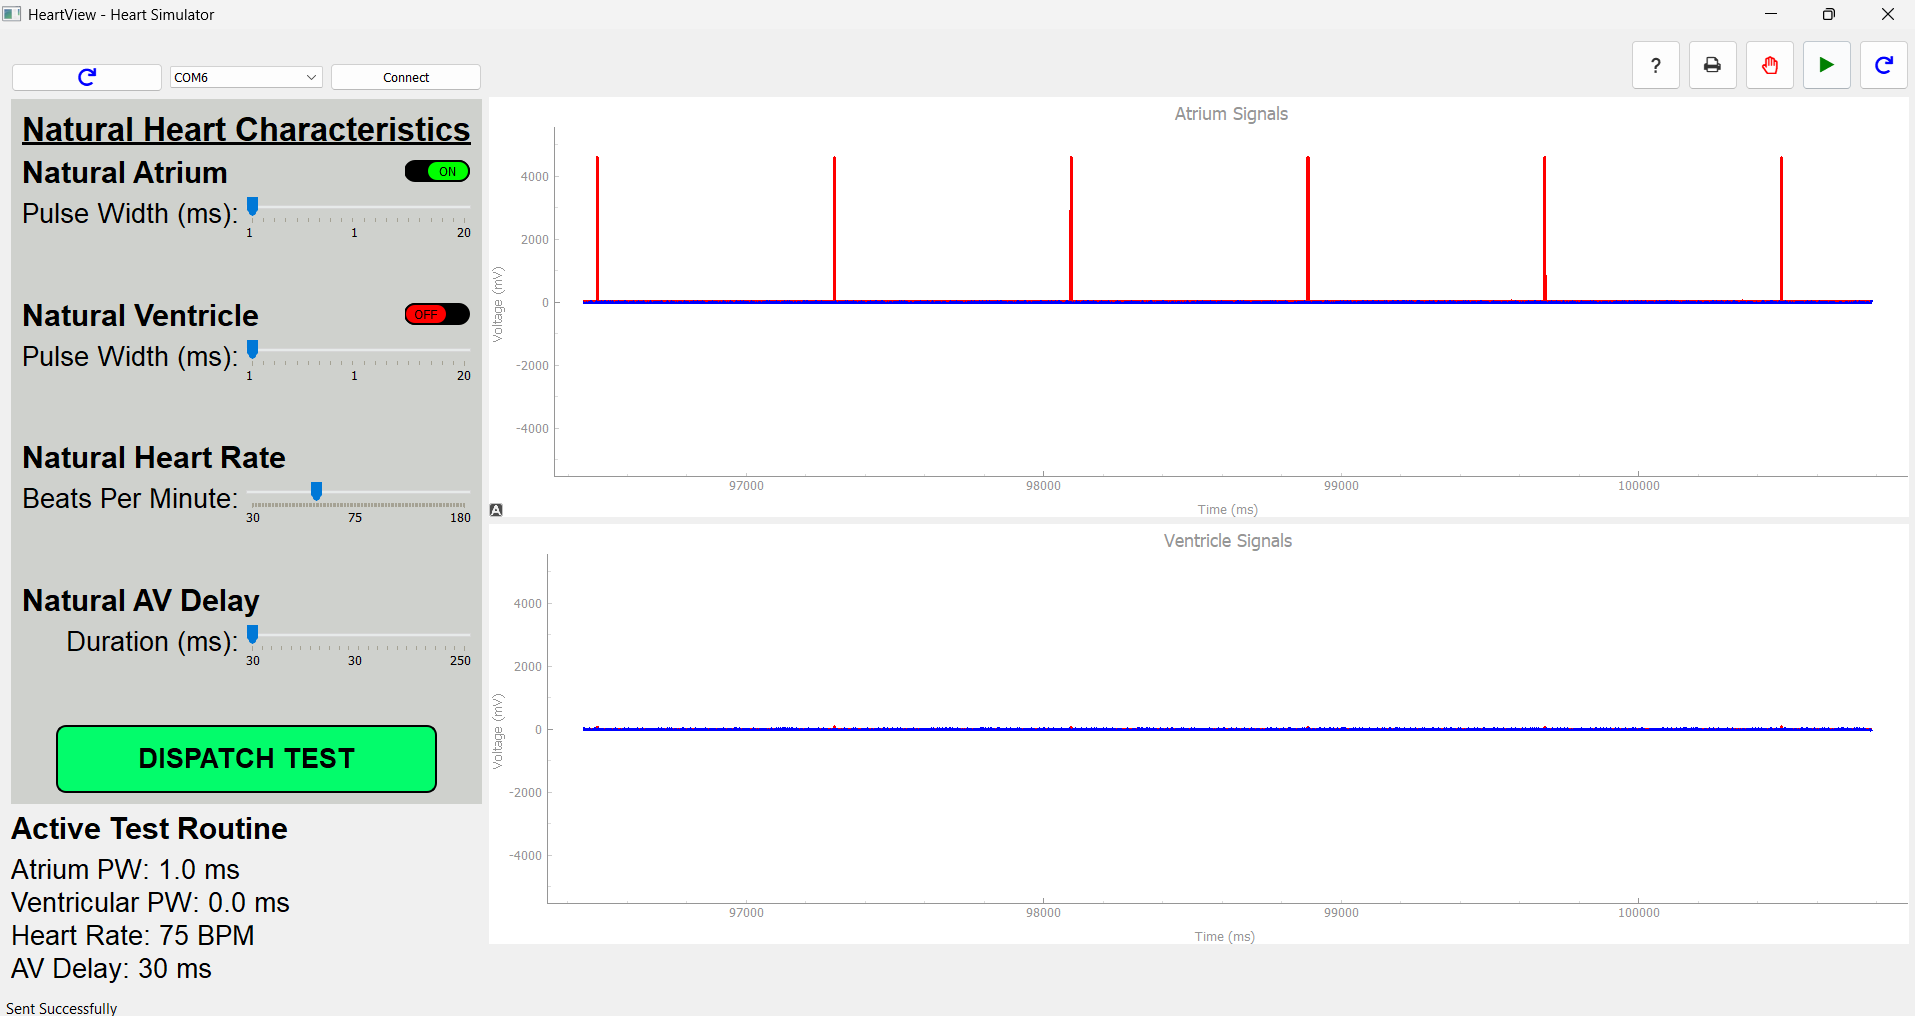
\includegraphics[width=\textwidth]{AAItest75.png}
        \caption{AAI Test 75 BPM}
    \end{figure}
\end{tcolorbox}

\newpage
\subsubsubsection{Testing of VVI}

\paragraph{No Natural Heart Rate}

\begin{enumerate}[label=]
   \item \textbf{Purpose:} The purpose of this test is to test basic VVI functionality with no inputted heart rate.
   \item \textbf{Input Conditions:} General inputs of mode = 3, VVI, and hysteresis = 0, off, standard ventricle 
   inputs, and monitored ventricle pulses.
   \item \textbf{Expected Output:} Consistent, evenly spaced pulses in the output.
   \item \textbf{Actual Output:} Output of testing is exactly that of expected, as shown below in \hyperref[VVItestnor]{Figure 17}.
   \item \textbf{Result:} Pass
\end{enumerate}

\begin{tcolorbox}
    \begin{figure}[H]\label{VVItestnor}
        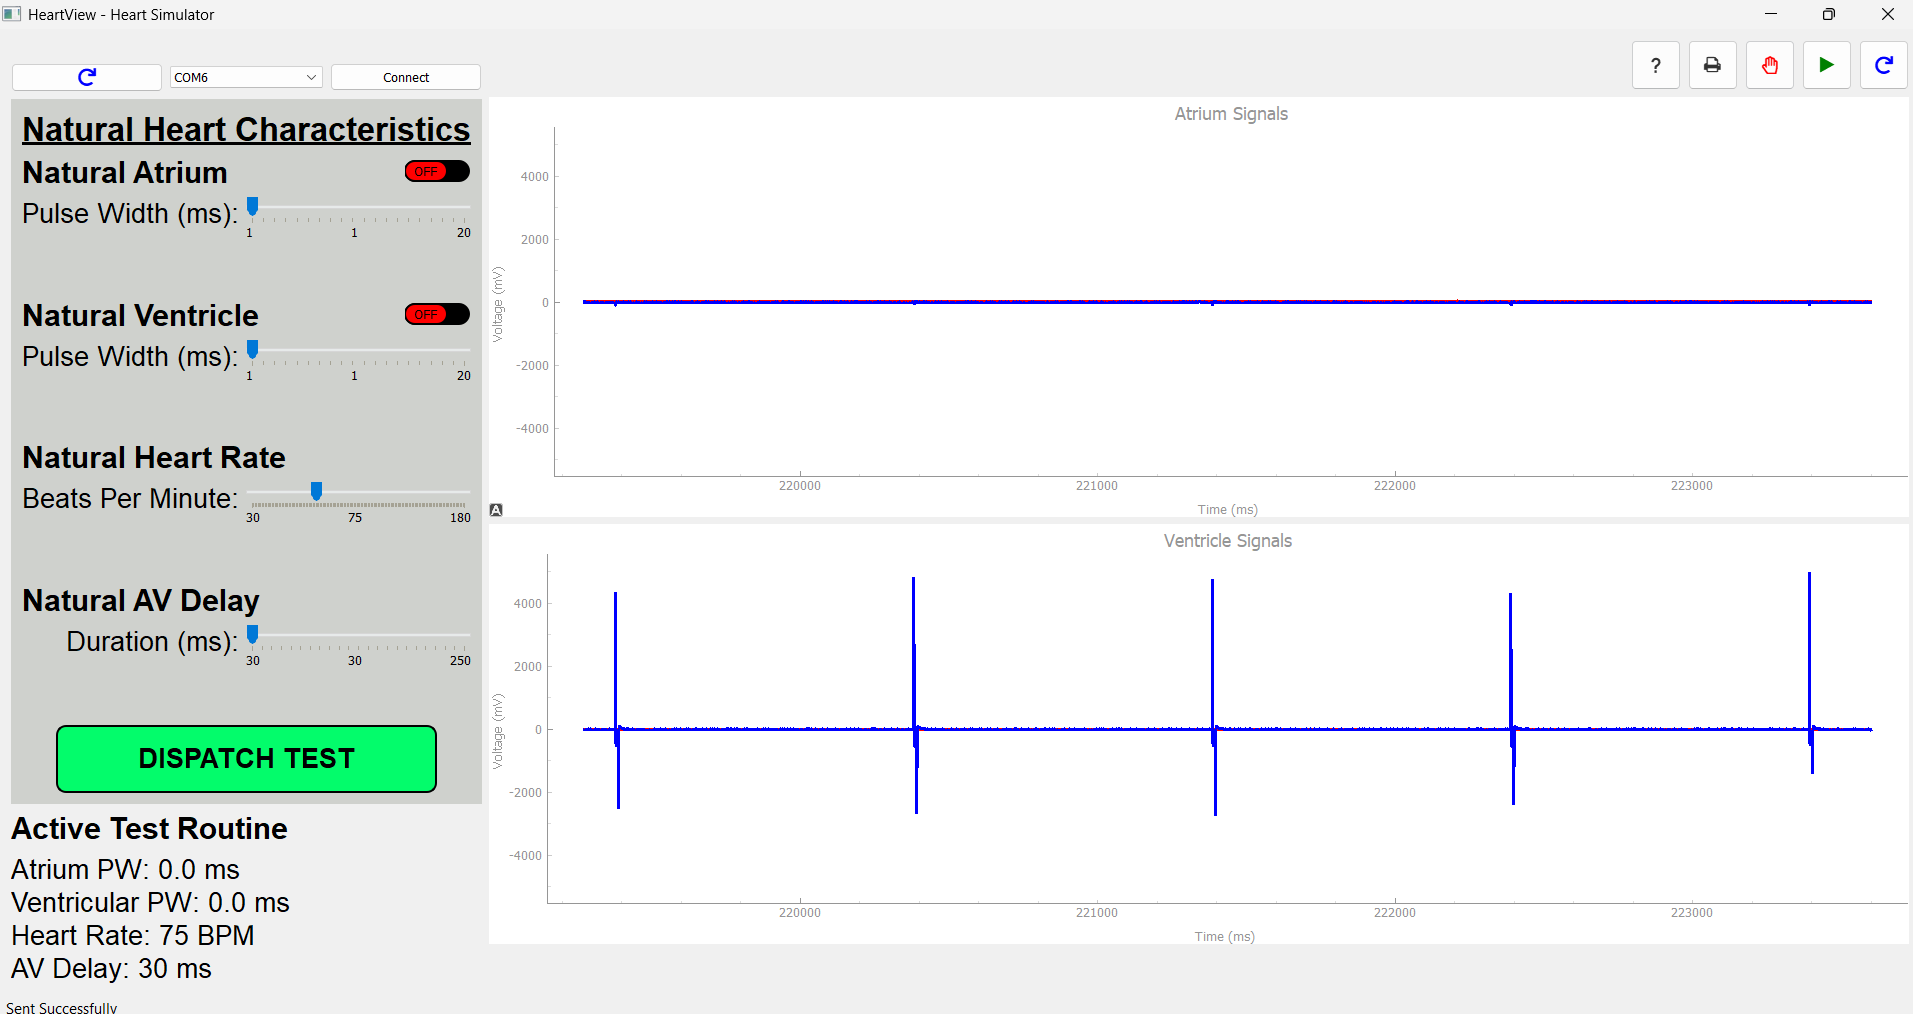
\includegraphics[width=\textwidth]{VVItestnohr.png}
        \caption{VVI Test No Heart Rate}
    \end{figure}
\end{tcolorbox}

\newpage
\paragraph{Natural Heart Rate at 45 BPM}

\begin{enumerate}[label=]
   \item \textbf{Purpose:} The purpose of this test is to test basic VVI functionality with no inputted heart rate.
   \item \textbf{Input Conditions:} General inputs of mode = 3, VVI, and hysteresis = 0, off, standard ventricle 
   inputs, and monitored ventricle pulses.
   \item \textbf{Expected Output:} The pacemaker should pulse after the refactory period expires. An output of blue pulses right before the natural 
   red pulses is expected.
   \item \textbf{Actual Output:} Output of testing is exactly that of expected, as shown below in \hyperref[VVItest45]{Figure 18}.
   \item \textbf{Result:} Pass
\end{enumerate}

\begin{tcolorbox}
    \begin{figure}[H]\label{VVItest45}
        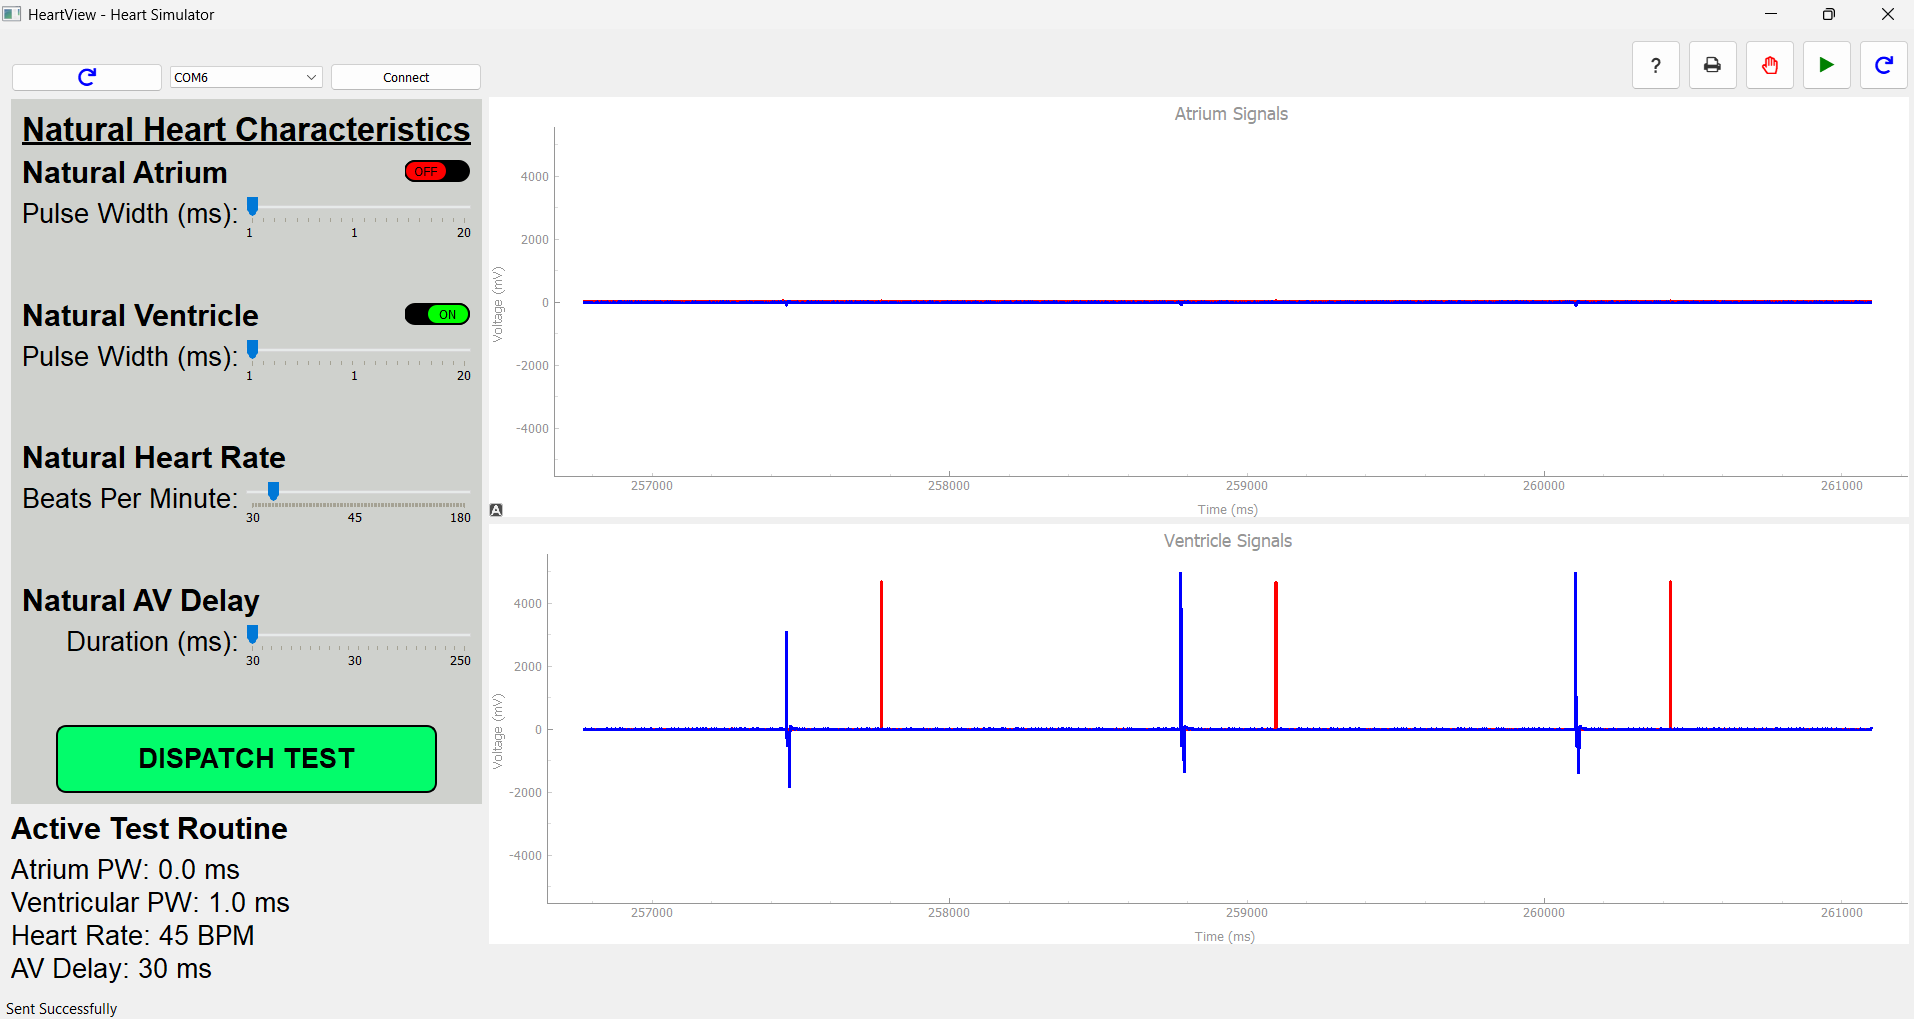
\includegraphics[width=\textwidth]{VVItest35.png}
        \caption{VVI Test 45 BPM}
        
    \end{figure}
\end{tcolorbox}

\newpage
\paragraph{Natural Heart Rate at 75 BPM}

\begin{enumerate}[label=]
   \item \textbf{Purpose:} The purpose of this test is to test basic VVI functionality with no inputted heart rate.
   \item \textbf{Input Conditions:} General inputs of mode = 3, VVI, and hysteresis = 0, off, standard ventricle 
   inputs, and monitored ventricle pulses.
   \item \textbf{Expected Output:} As a nominal heart reate is being inputted, the pacemaker should not be delivering pacing pulses 
   as the simulated heart rate is nominal and healthy.
   \item \textbf{Actual Output:} Output of testing is exactly that of expected, as shown below in \hyperref[VVItest45]{Figure 18}.
   \item \textbf{Result:} Pass
\end{enumerate}

\begin{tcolorbox}
    \begin{figure}[H]\label{VVItest75}
        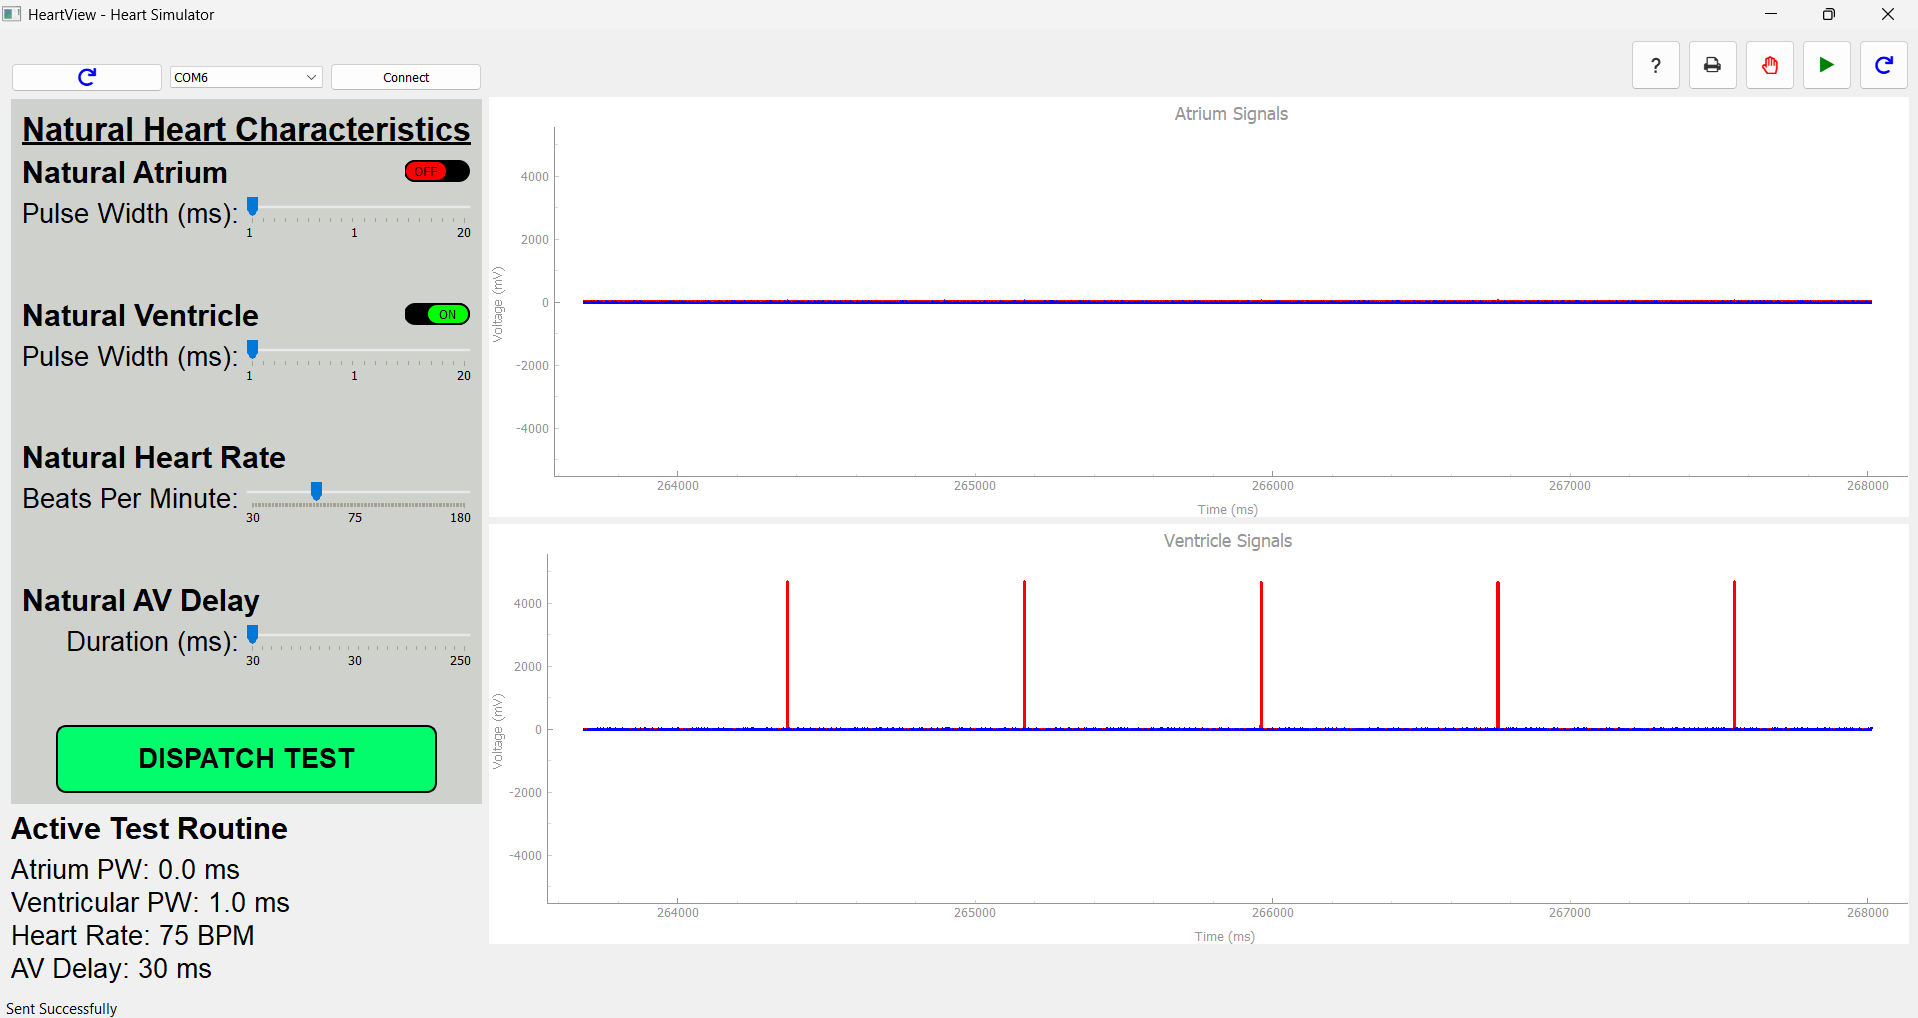
\includegraphics[width=\textwidth]{VVItest75.png}
        \caption{VVI Test 75 BPM}
    \end{figure}
\end{tcolorbox}

\newpage
\subsubsubsection{Hysteresis Testing}

\paragraph{Hysteresis Test 1 (60 BPM)}

\begin{enumerate}[label=]
   \item \textbf{Purpose:} The purpose of this test is to test basic hysteresis mode functionality.
   \item \textbf{Input Conditions:} General inputs of mode = 2, AAI, and hysteresis = 1, on, standard atrium 
   inputs, and monitored atrial pulses at 50 BPM.
   \item \textbf{Expected Output:} No output of the pacemaker.
   \item \textbf{Actual Output:} Output of testing is exactly that of expected, as shown below in \hyperref[Hystest1]{Figure 20}.
   \item \textbf{Result:} Pass
\end{enumerate}

\begin{tcolorbox}
    \begin{figure}[H]\label{Hystest1}
        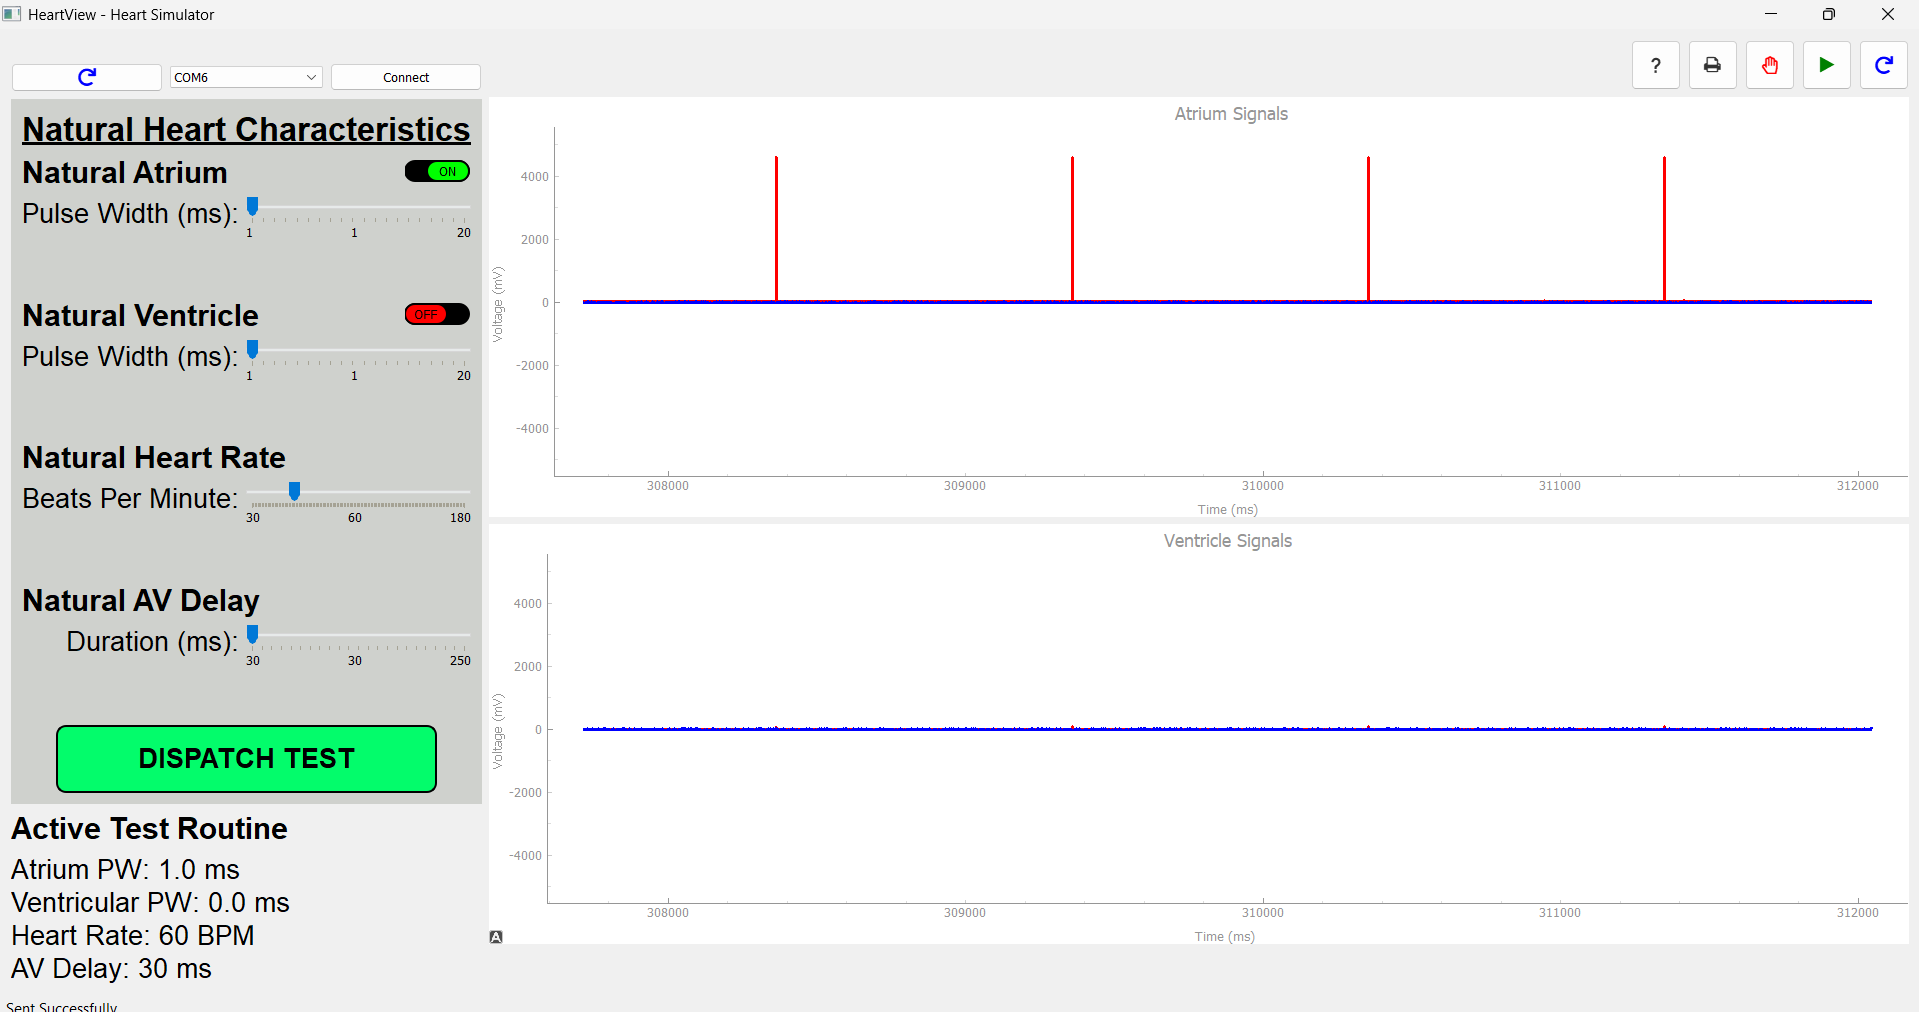
\includegraphics[width=\textwidth]{hystherisistest.png}
        \caption{Hysterisis Test 1}
    \end{figure}
\end{tcolorbox}

\newpage
\paragraph{Hysteresis Test 2 (50 BPM)}

\begin{enumerate}[label=]
   \item \textbf{Purpose:} The purpose of this test is to test basic hysteresis mode functionality.
   \item \textbf{Input Conditions:} General inputs of mode = 2, AAI, and hysteresis = 1, on, standard atrium 
   inputs, and monitored atrial pulses at 50 BPM.
   \item \textbf{Expected Output:} No output of the pacemaker.
   \item \textbf{Actual Output:} Output of testing is exactly that of expected, as shown below in \hyperref[Hystest2]{Figure 21}.
   \item \textbf{Result:} Pass
\end{enumerate}

\begin{tcolorbox}
    \begin{figure}[H]\label{Hystest2}
        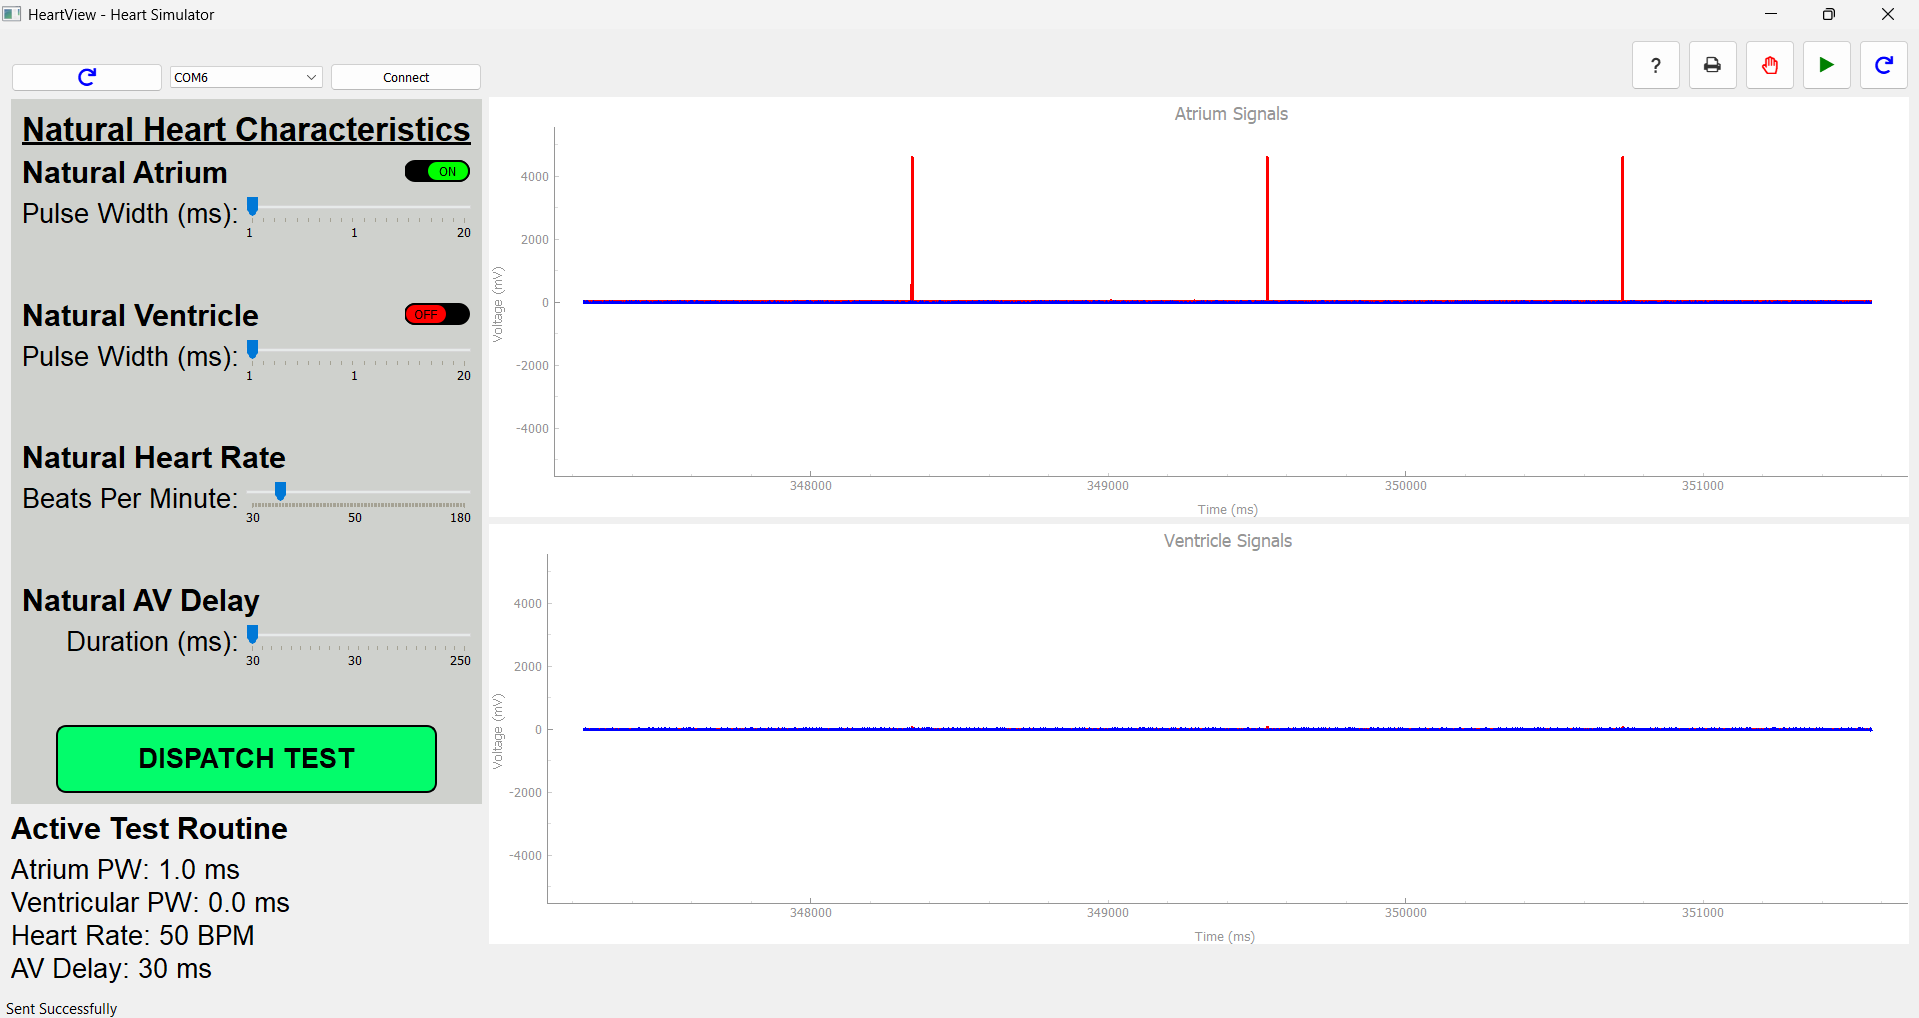
\includegraphics[width=\textwidth]{hythersistest2.png}
        \caption{Hysterisis Test 2}
    \end{figure}
\end{tcolorbox}

\newpage
\paragraph{Hysteresis Test 3 (40 BPM)}

\begin{enumerate}[label=]
   \item \textbf{Purpose:} The purpose of this test is to test basic hysteresis mode functionality.
   \item \textbf{Input Conditions:} General inputs of mode = 2, AAI, and hysteresis = 1, on, standard atrium 
   inputs, and monitored atrial pulses at 50 BPM.
   \item \textbf{Expected Output:} Delayed output signals from the pacemaker.
   \item \textbf{Actual Output:} Output of testing is exactly that of expected, as shown below in \hyperref[Hystest3]{Figure 22}.
   \item \textbf{Result:} Pass
\end{enumerate}

\begin{tcolorbox}
    \begin{figure}[H]\label{Hystest3}
        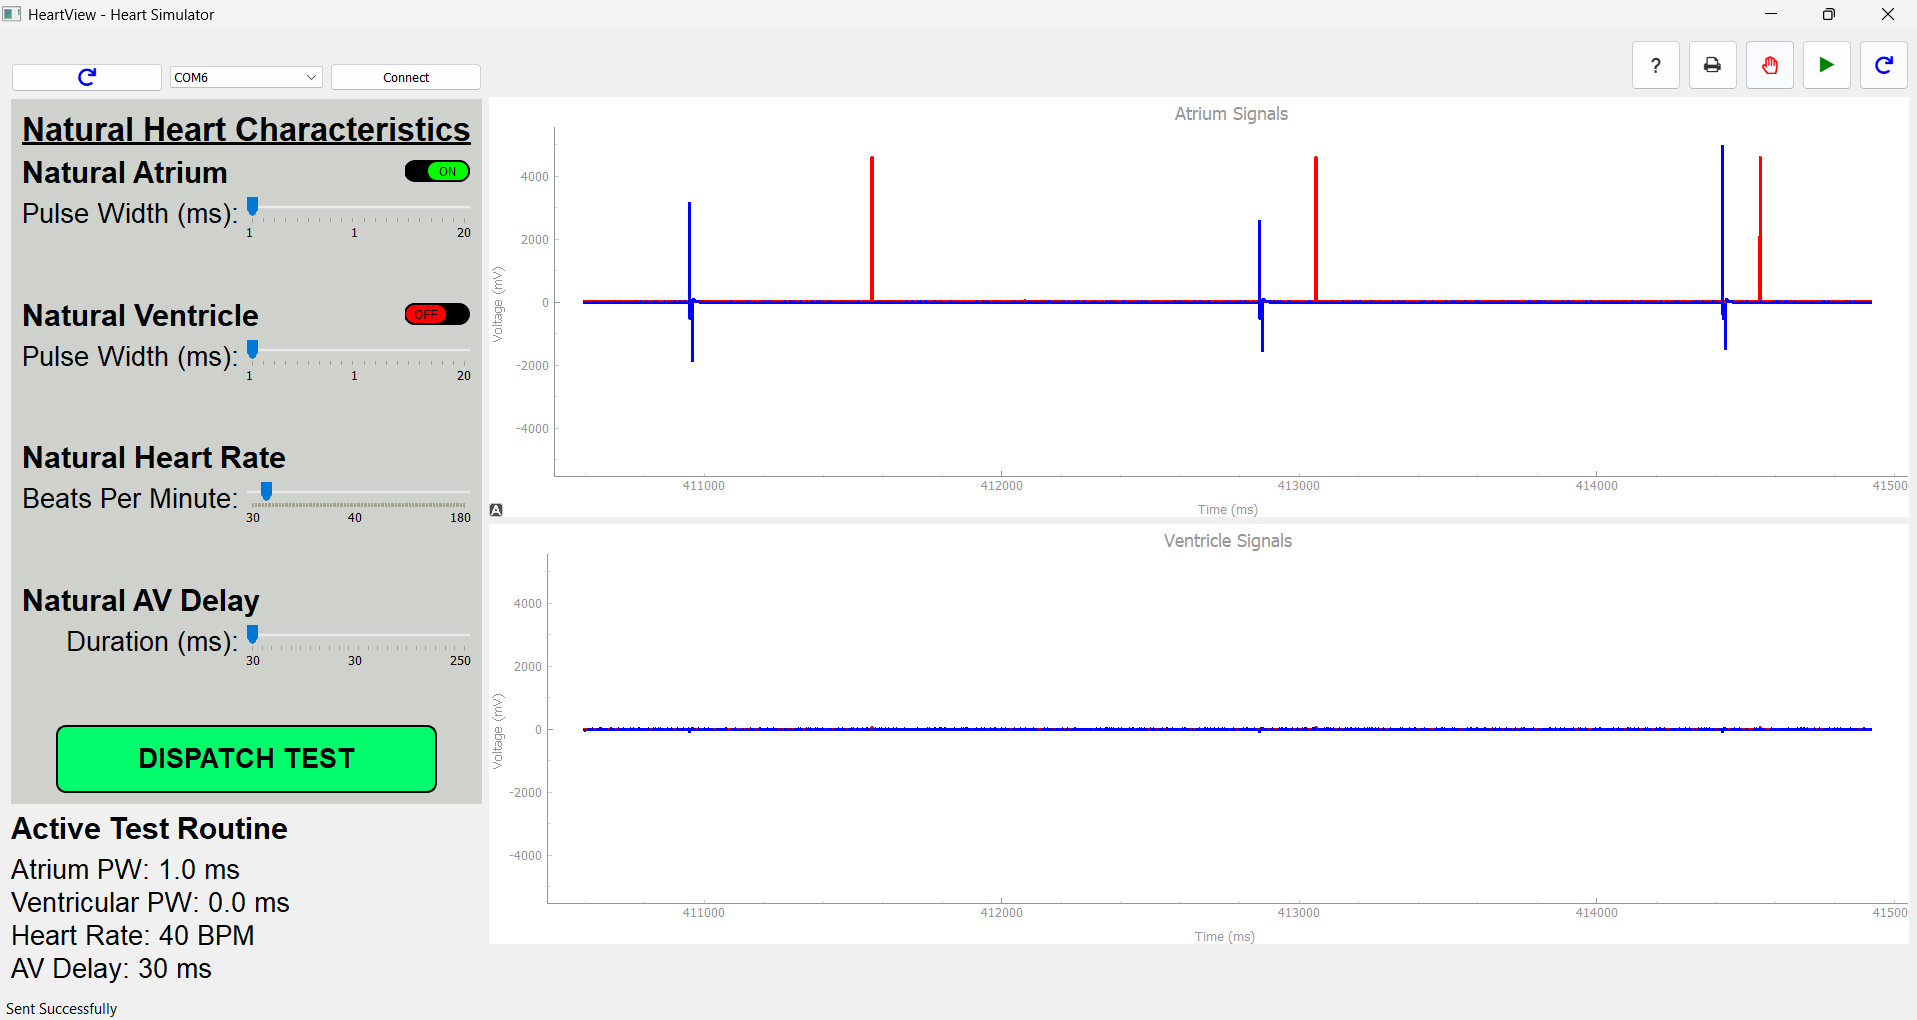
\includegraphics[width=\textwidth]{hytheresistest3.png}
        \caption{Hysterisis Test 3}
    \end{figure}
\end{tcolorbox}

\newpage
\subsubsection{DCM Testing}

\subsubsubsection{Login and Registration}

\begin{enumerate}[label=]
   \item \textbf{Purpose:} The purpose of this test is to verify correct storage of newly registered user data 
   and allow login. 
   \item \textbf{Input Conditions:} A random username and password. This will be used again in the login screen to access the DCM. 
   \item \textbf{Expected Output:} A window should pop up notifying the user an account has been registered. The 
   DCM controls should be accessible after the user logs in. 
   \item \textbf{Actual Output:} Dialogue is shown and the file is updated to include new user data. The user is then brought to the 
   \item \textbf{Result:} Pass
\end{enumerate}

\begin{tcolorbox}
    \begin{figure}[H]\label{regtest}
        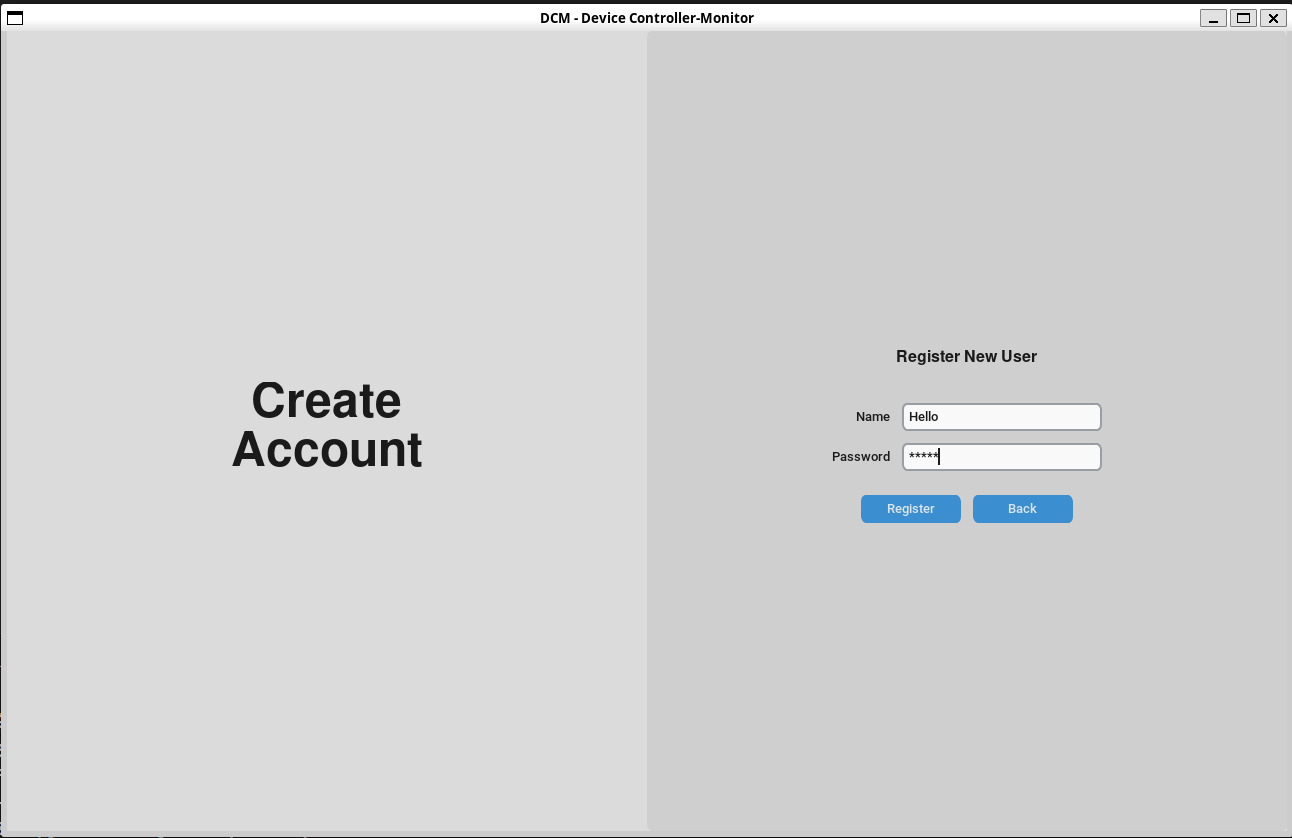
\includegraphics[width=\textwidth]{registertest.png}
        \caption{Registration Test}
    \end{figure}
\end{tcolorbox}

\begin{tcolorbox}
    \begin{figure}[H]\label{regres}
        \centering
        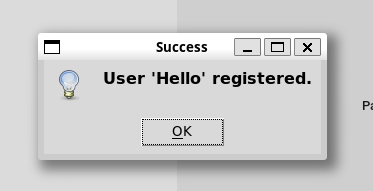
\includegraphics[width=0.9\textwidth]{registerres.png}
        \caption{Registration Result}
    \end{figure}
\end{tcolorbox}

\begin{tcolorbox}
    \begin{figure}[H]\label{logtest}
        \centering
        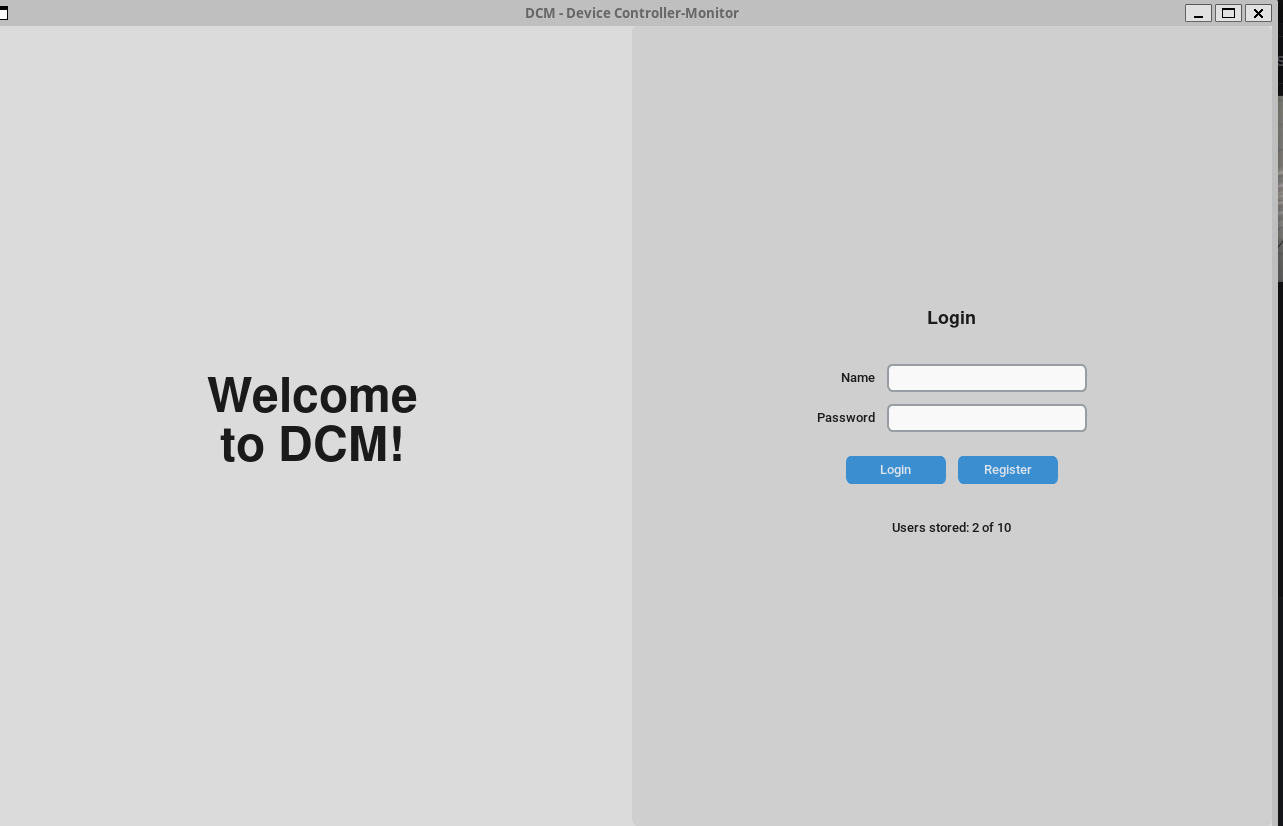
\includegraphics[width=0.9\textwidth]{logintest.png}
        \caption{Login Test}
    \end{figure}
\end{tcolorbox}

\begin{tcolorbox}
    \begin{figure}[H]\label{logres}
        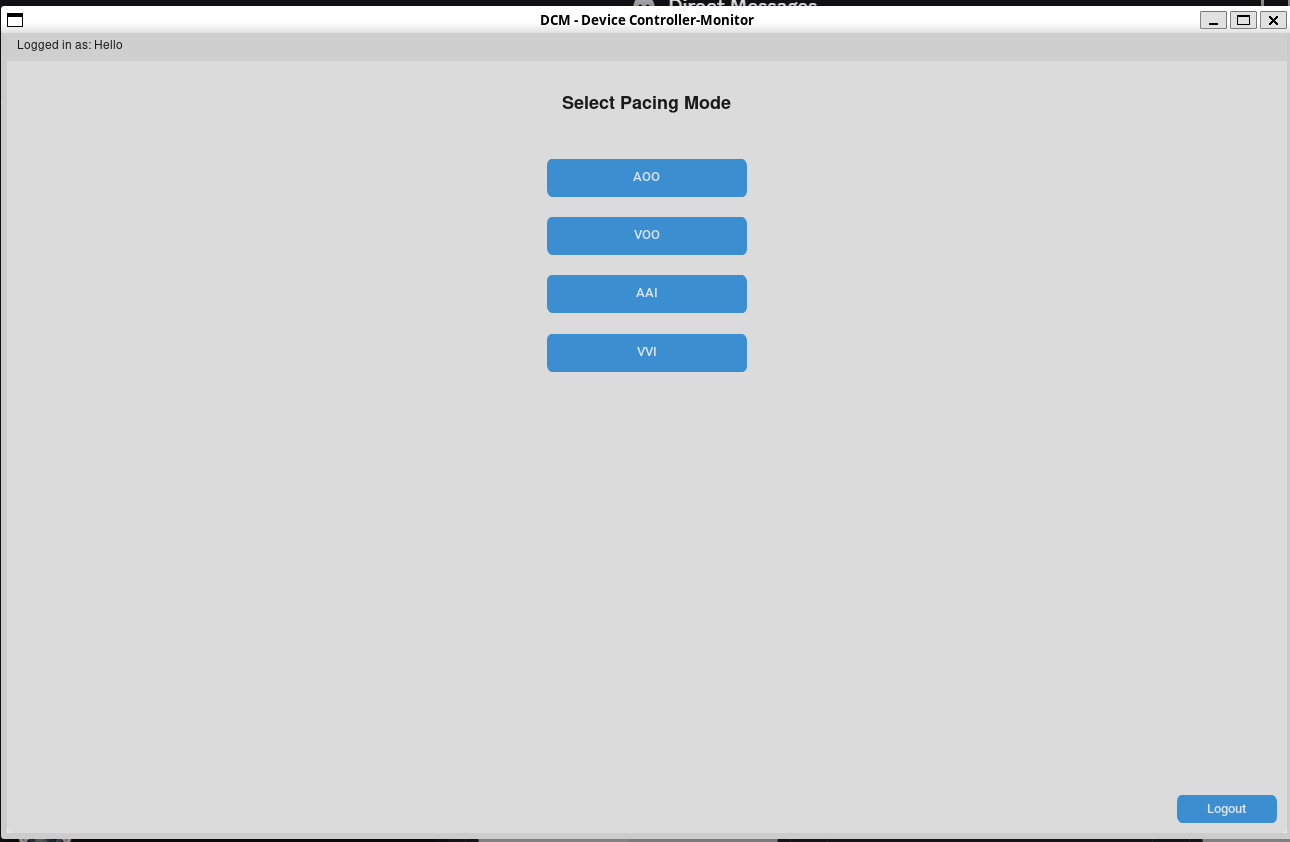
\includegraphics[width=\textwidth]{loginres.png}
        \caption{Login Result}
    \end{figure}
\end{tcolorbox}

\newpage
\subsubsubsection{Parameter Input Validation}
\begin{enumerate}[label=]
   \item \textbf{Purpose:} To enforce numeric types within an allowed range and to ensure the upper rate interval is greater than lower rate interval. 
   \item \textbf{Input Conditions:} Entering a non-numeric, an out of range number and an upper rate interval that is greater than lower rate interval in parameter settings. 
   \item \textbf{Expected Output:} Invalid input dialogue is shown and parameter changes are not saved.
   \item \textbf{Actual Output:}  
   \item \textbf{Result:} Pass
\end{enumerate}


The below figures show the general parameter page with some values inputted as well as the results of putting 
invalid values into parameter page. 

\begin{tcolorbox}
    \begin{figure}[H]\label{genparam}
        \centering
        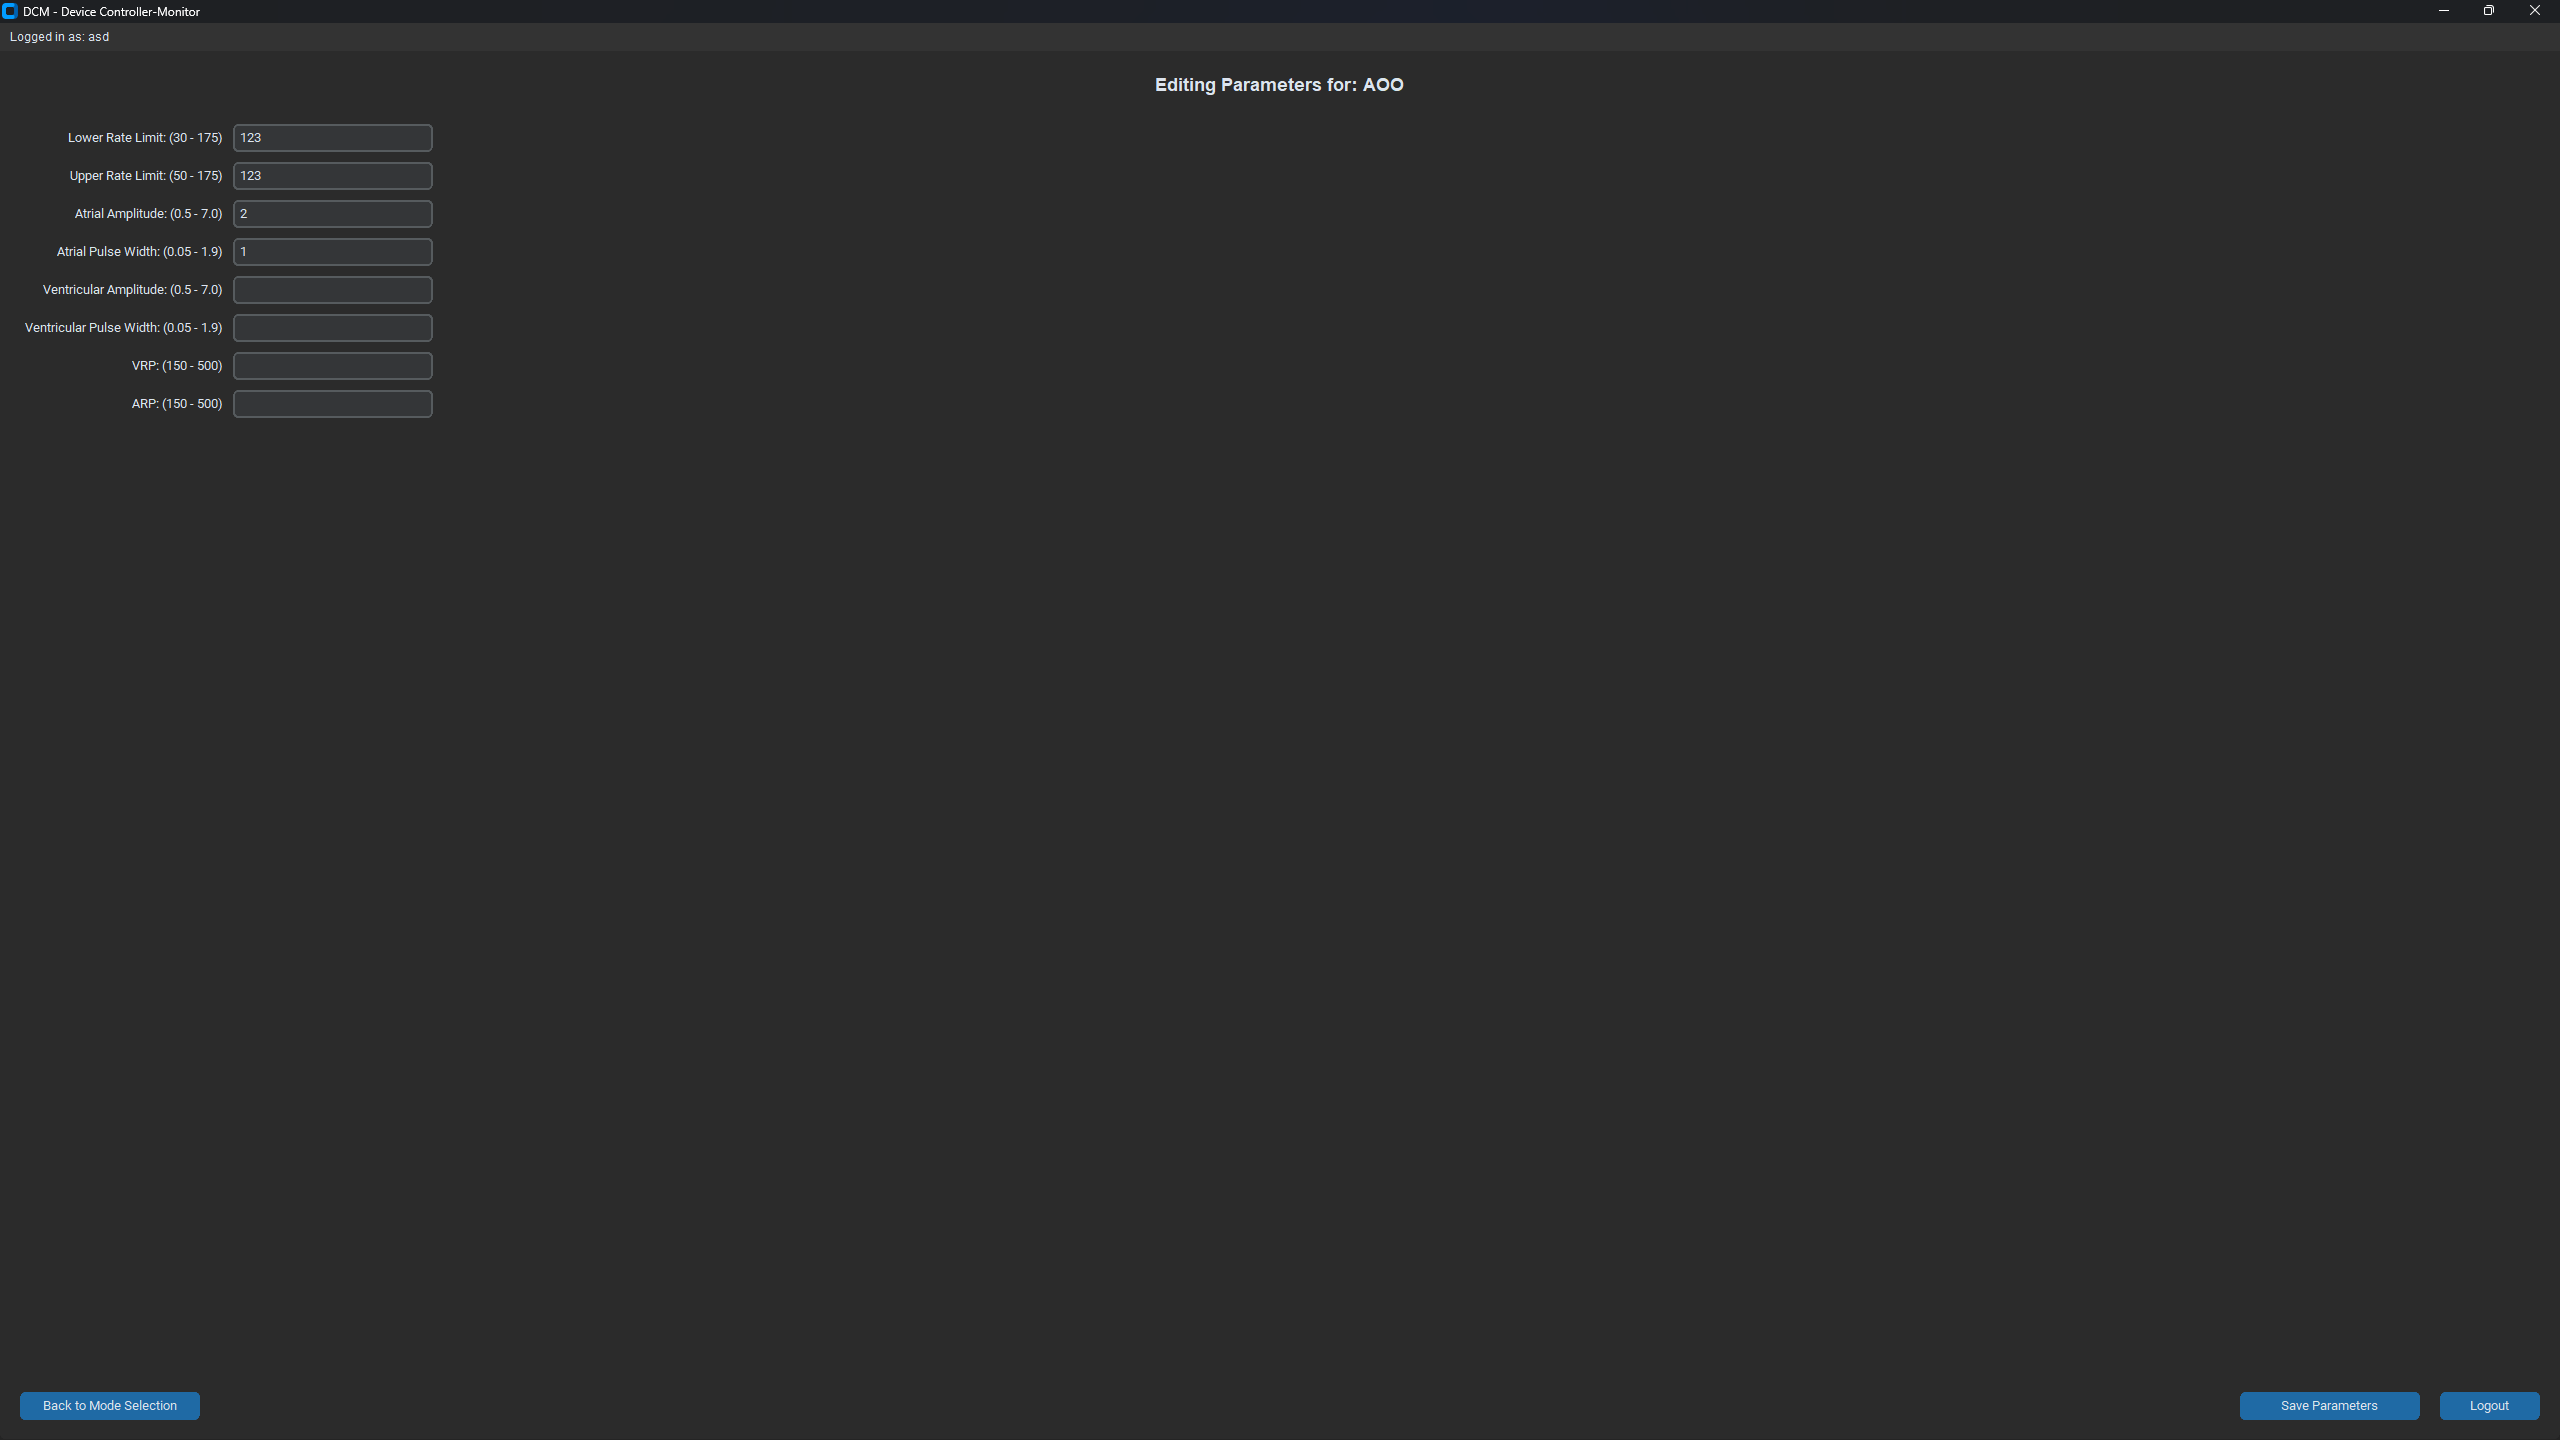
\includegraphics[width=\textwidth]{genparams.png}
        \caption{DCM Parameter Page with Values Filled}
    \end{figure}
\end{tcolorbox}

\begin{tcolorbox}
    \begin{figure}[H]\label{rangeparam}
        \centering
        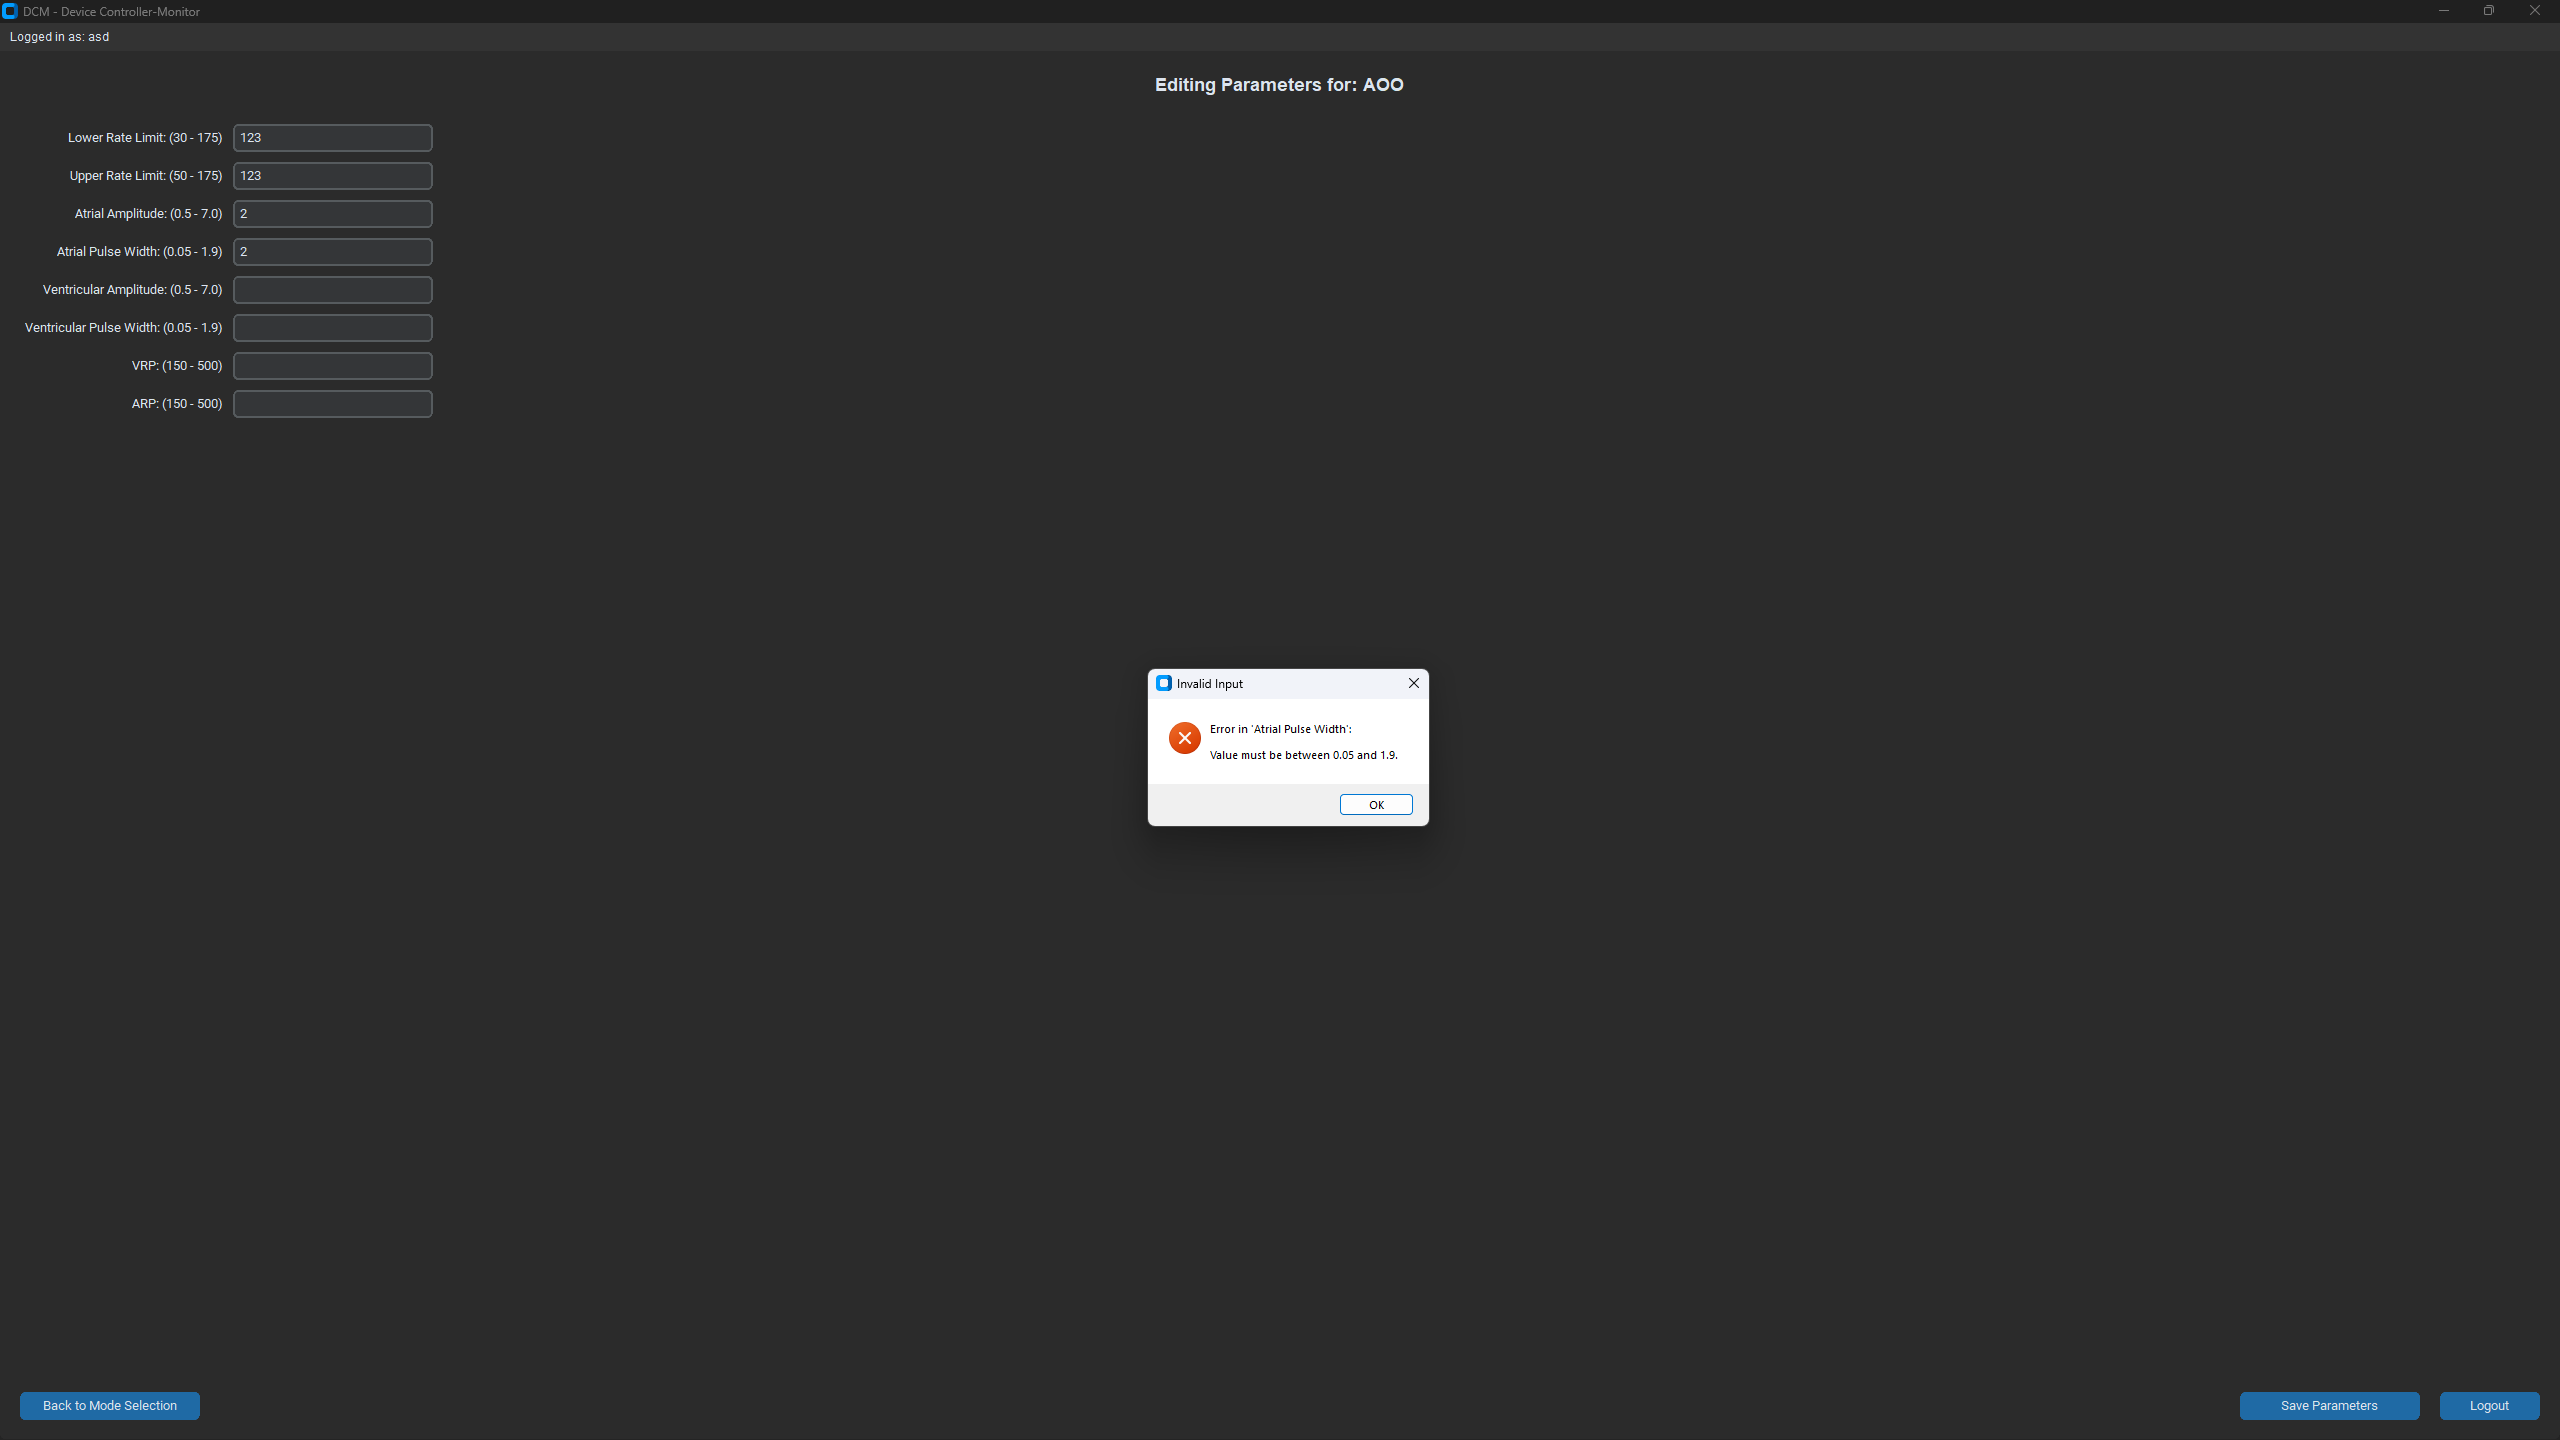
\includegraphics[width=0.9\textwidth]{rangeparam.png}
        \caption{DCM Parameter Error When Number Inputted is Out of Range}
    \end{figure}
\end{tcolorbox}


\begin{tcolorbox}
    \begin{figure}[H]\label{numparam}
        \centering
        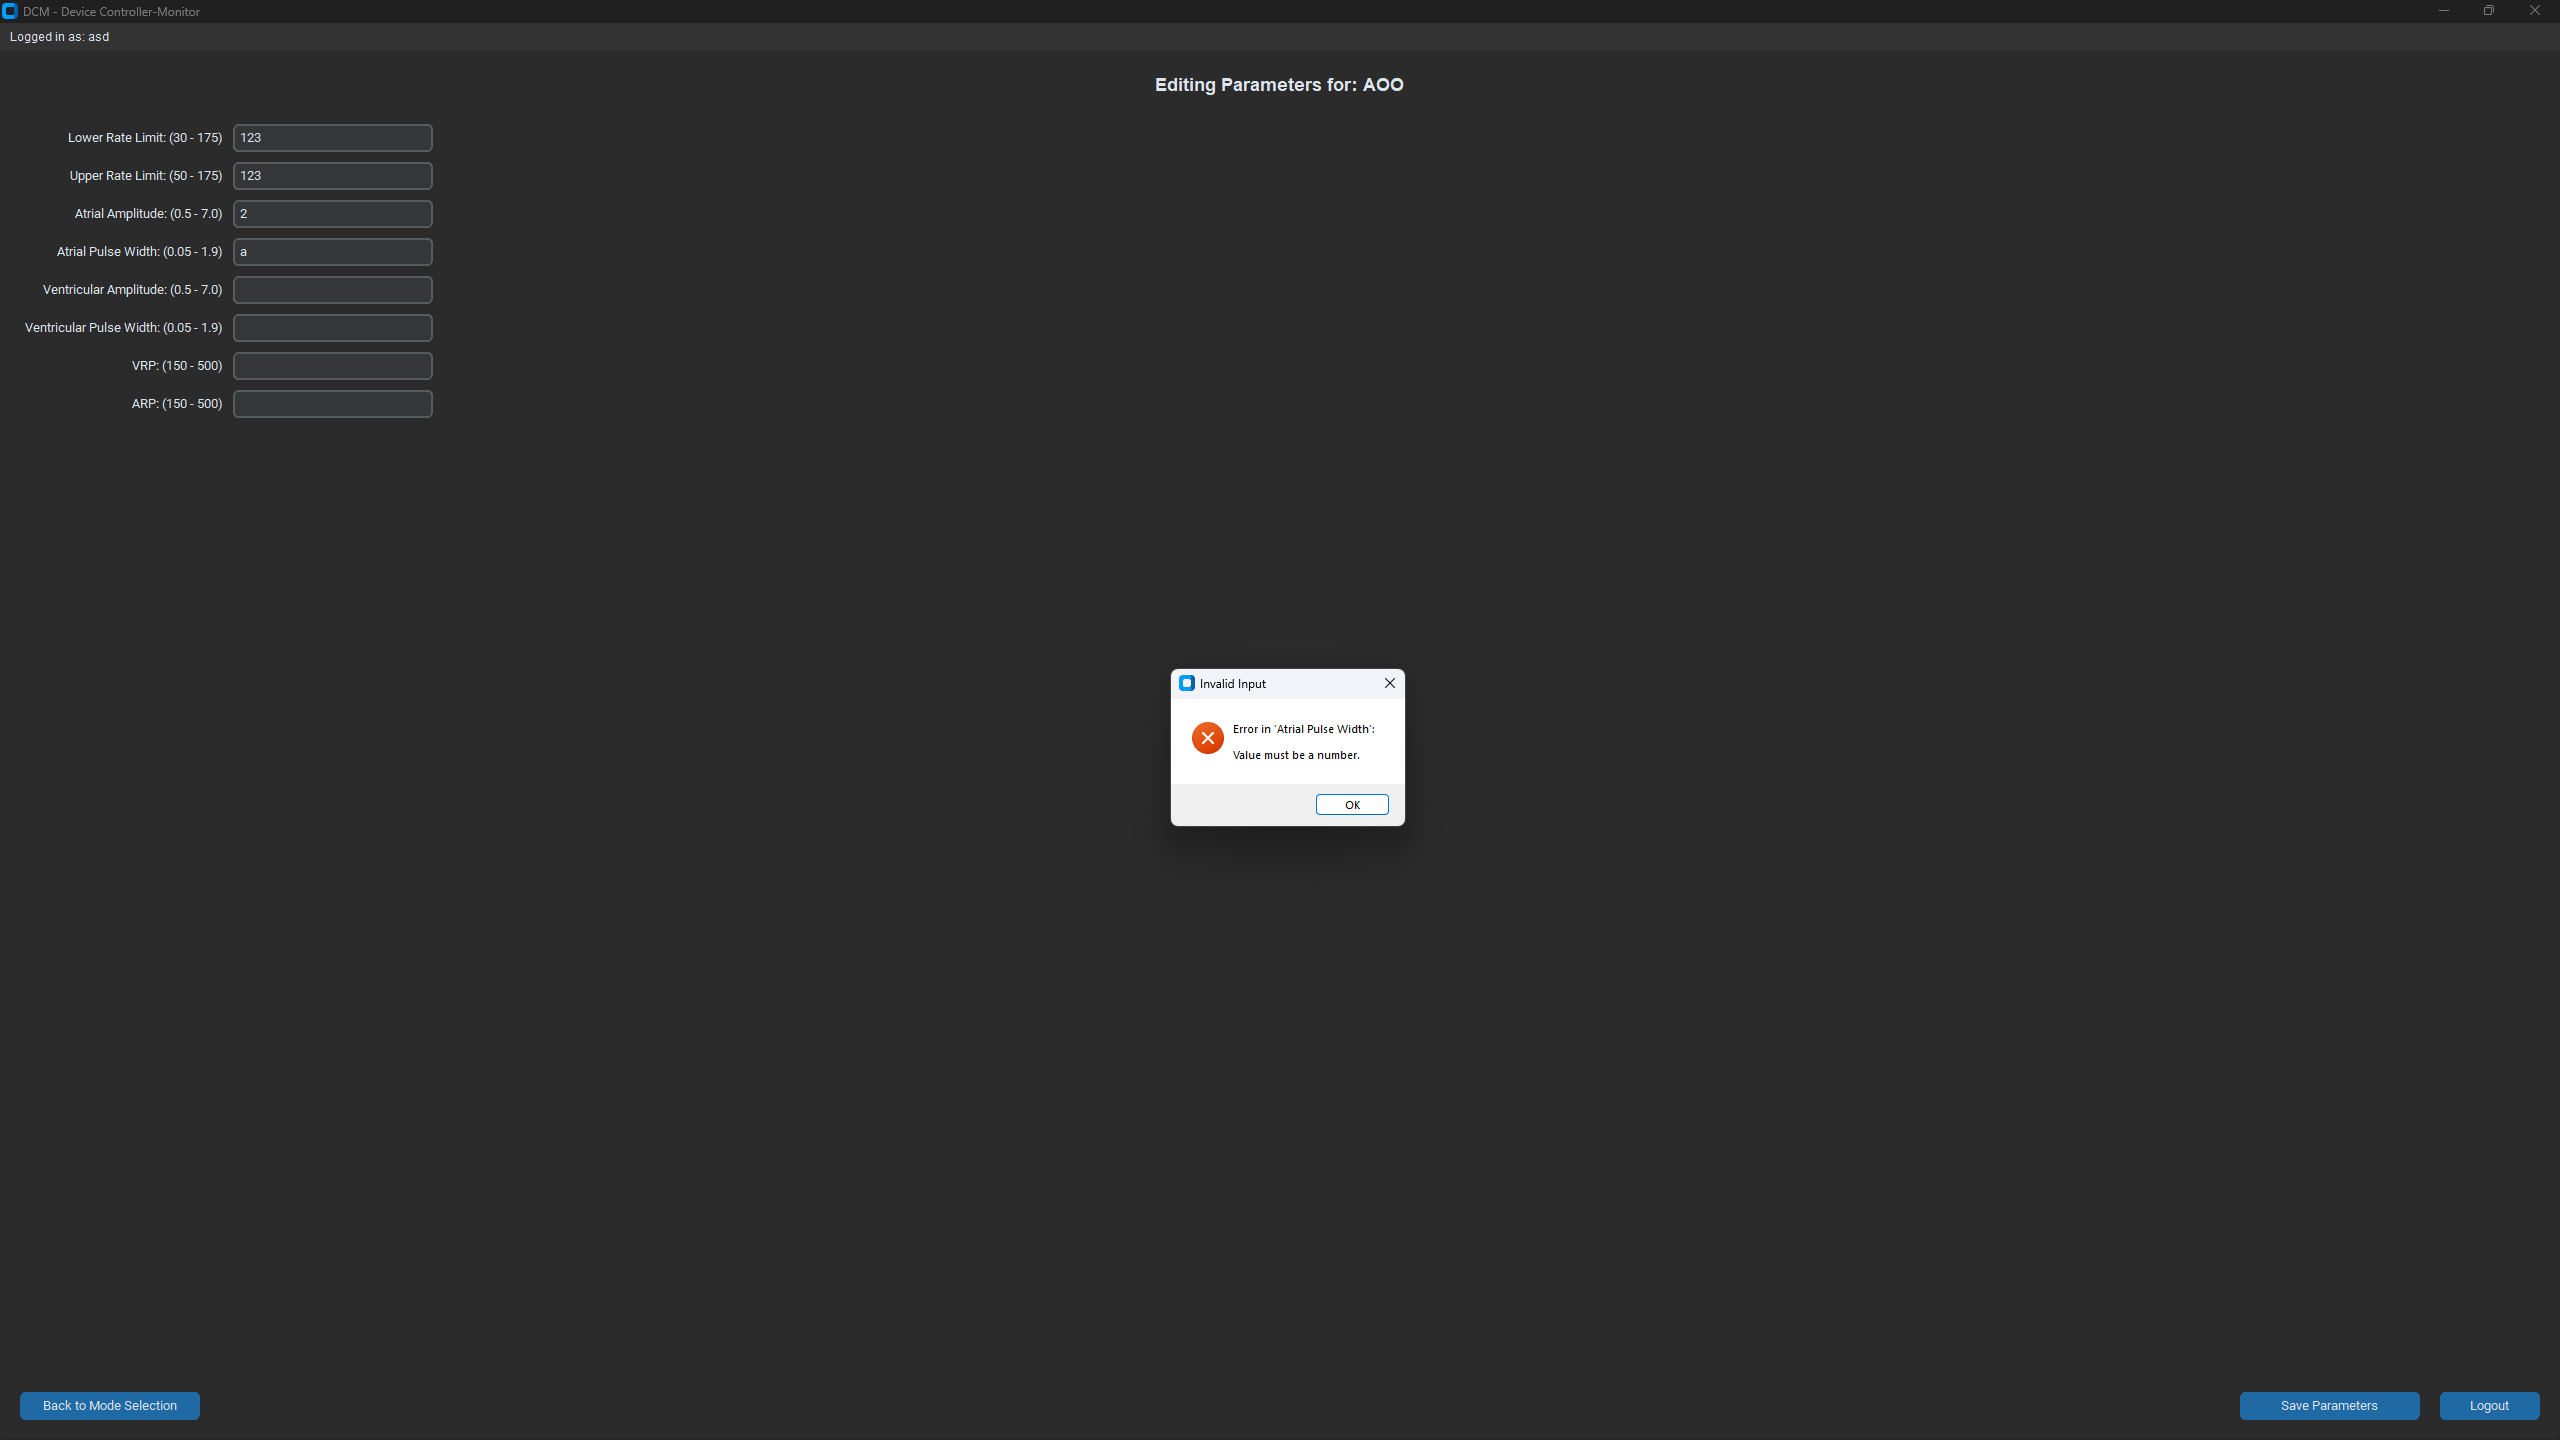
\includegraphics[width=0.9\textwidth]{numparam.png}
        \caption{DCM Parameter Error When Non-Number is Inputted}
    \end{figure}
\end{tcolorbox}

\begin{tcolorbox}
    \begin{figure}[H]\label{urlirl}
        \centering
        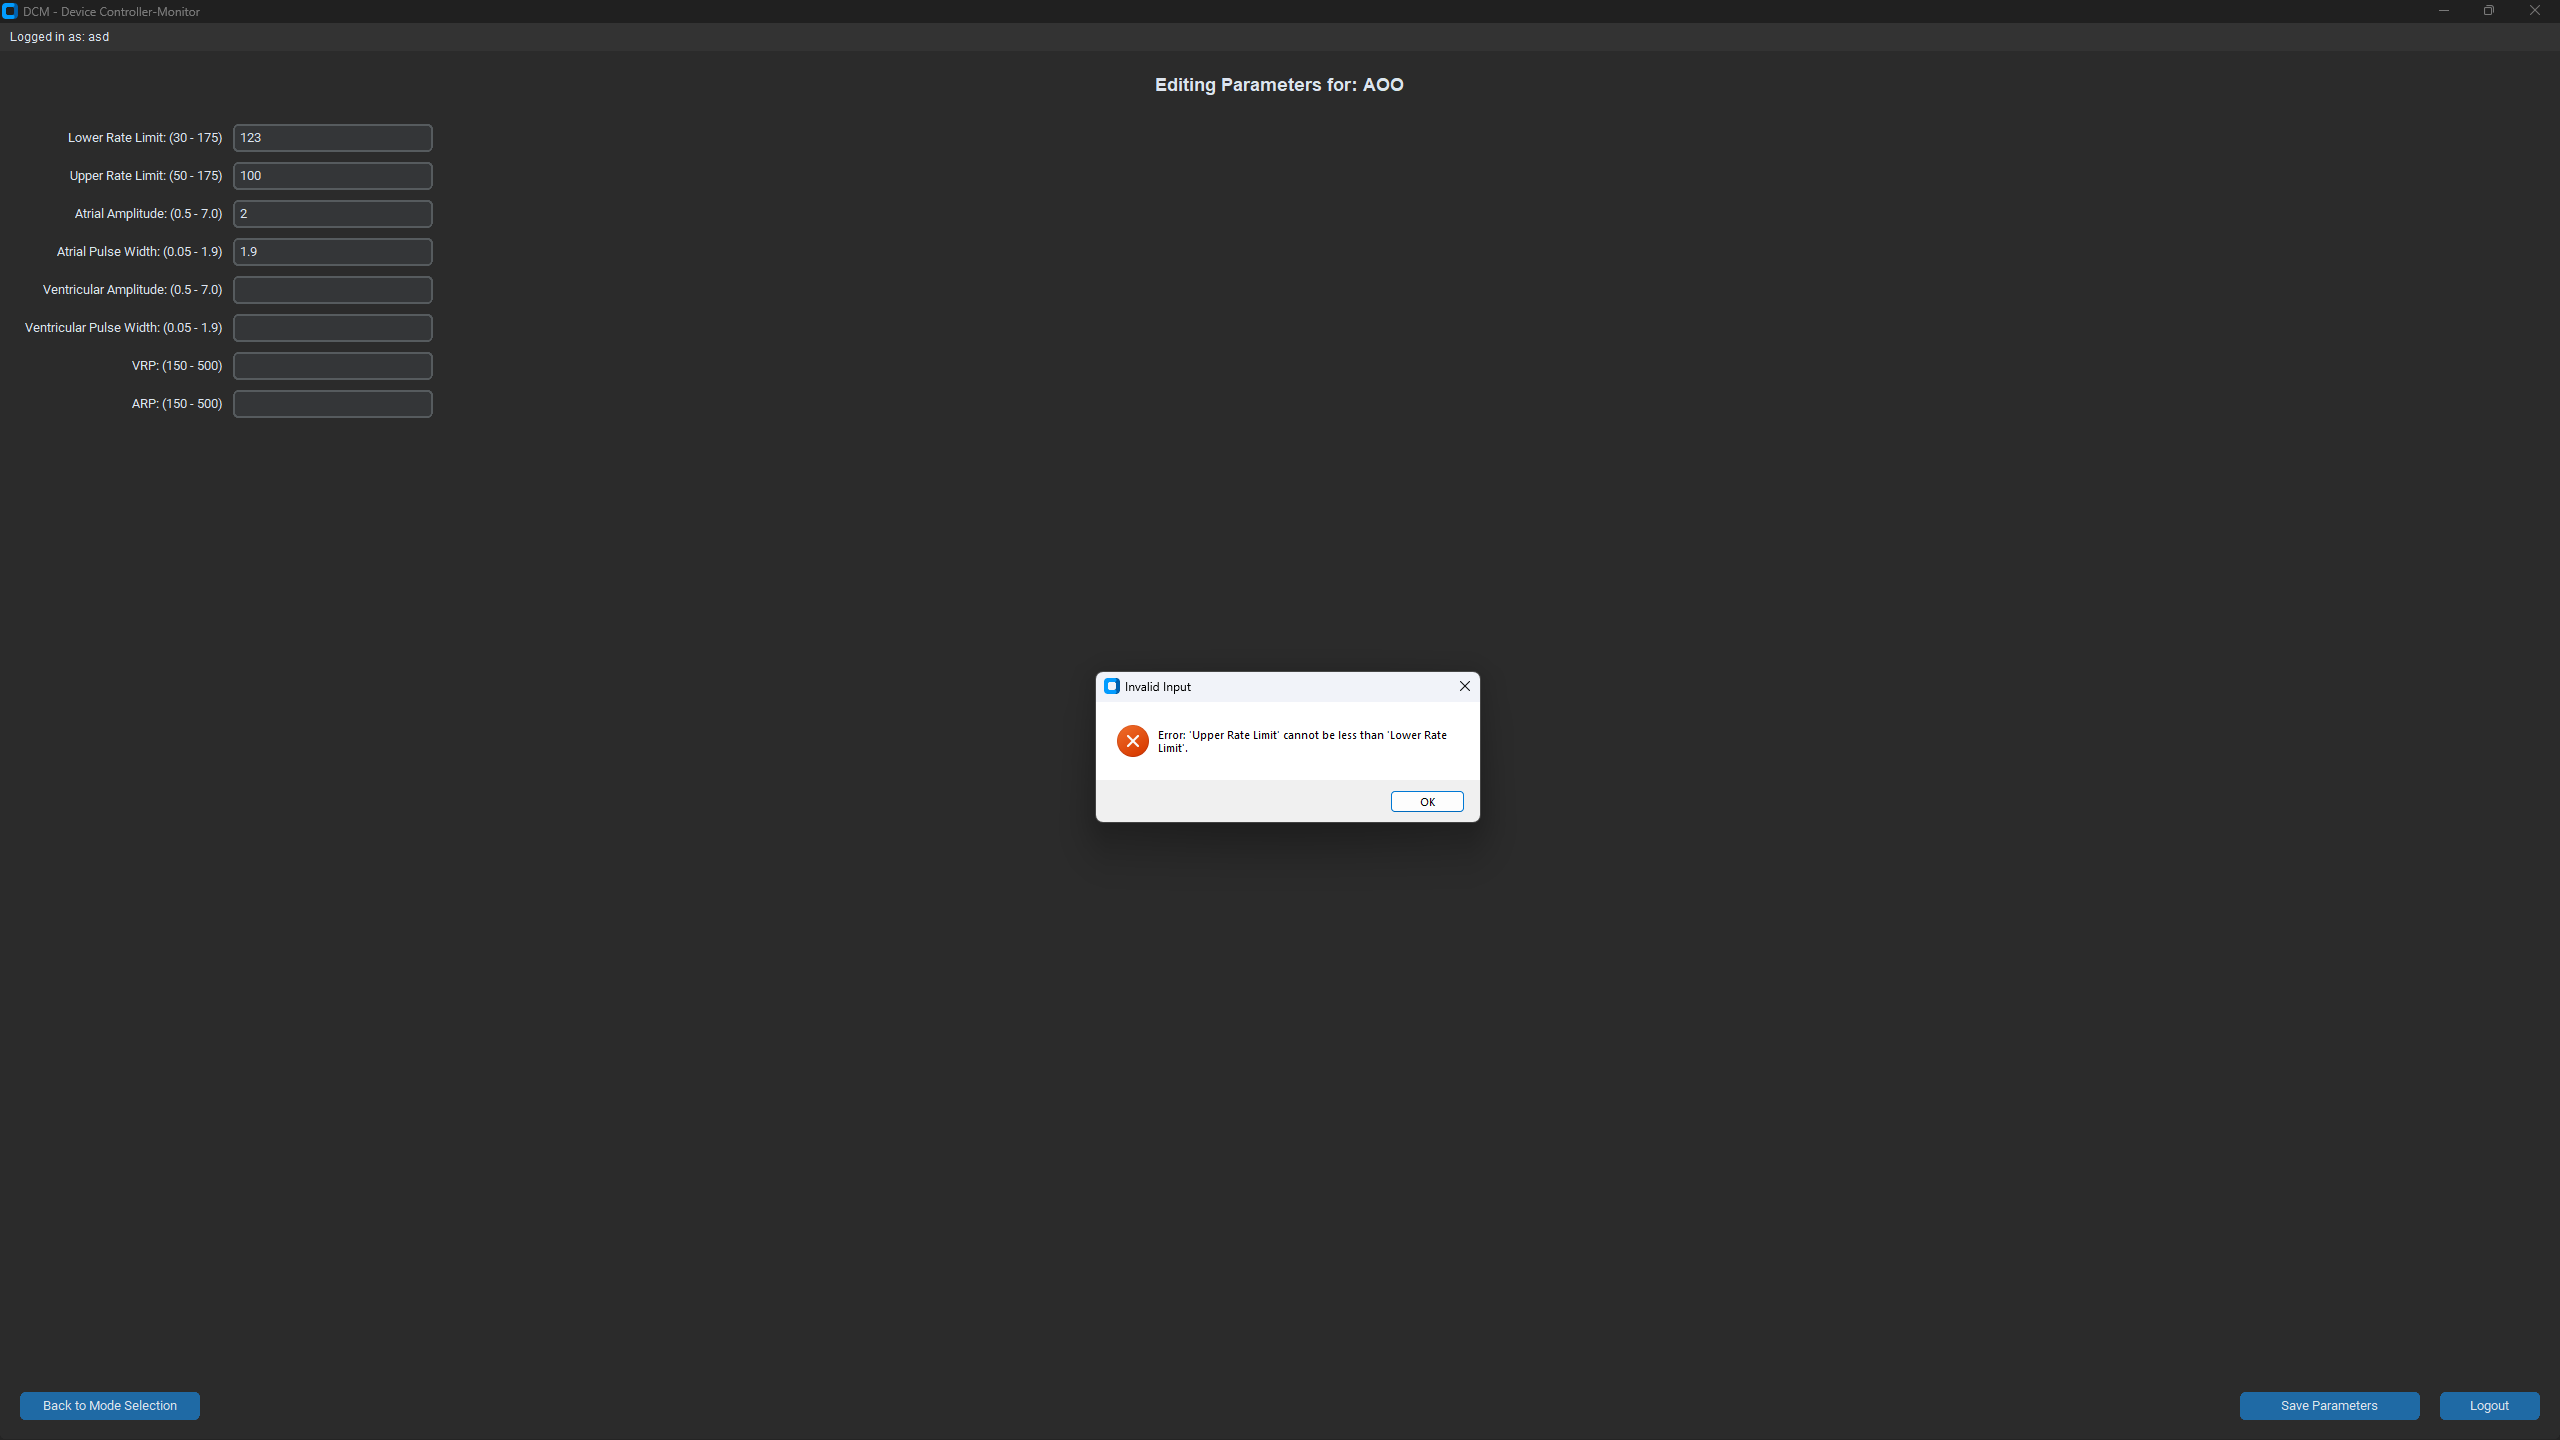
\includegraphics[width=0.9\textwidth]{urlirl.png}
        \caption{DCM Parameter Error When URL is Larger Than IRL}
    \end{figure}
\end{tcolorbox}

\newpage
\subsubsubsection{Mode Selection and Data Retrieval}
\begin{enumerate}[label=]
   \item \textbf{Purpose:} To test data storage, ensuring proper saving of user data
   \item \textbf{Input Conditions:} Registering account, logging in, and saving parameters.
   \item \textbf{Expected Output:} User data is now found in the associated JSON files.
   \item \textbf{Actual Output:}  Registered user data and parameters are found in their respective JSON files.
   \item \textbf{Result:} Pass
\end{enumerate}

This test was done in conjunction to previous tests except with a different user registered. A user "asd" 
with password "asd" was used for faster log ins. The following images are of the JSON files and the saved parameters 
from the previous test. 

\begin{tcolorbox}
    \begin{figure}[H]\label{savedparams}
        \centering
        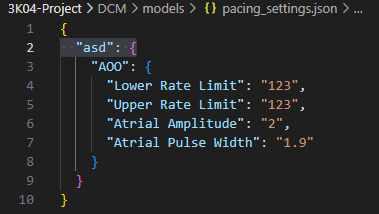
\includegraphics[width=0.8\textwidth]{savedparams.png}
        \caption{Stored Parameter File}
    \end{figure}
\end{tcolorbox}

\begin{tcolorbox}
    \begin{figure}[H]\label{saveduser}
        \centering
        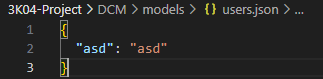
\includegraphics[width=0.8\textwidth]{saveduser.png}
        \caption{Stored Users File}
    \end{figure}
\end{tcolorbox}



\newpage
\subsection{GenAI Usage}

We used a Generative AI assistant to support development of the DCM. It provided starter boilerplate for a 
Tkinter app with a welcome screen, registration and login, JSON storage capped at ten users, which we then 
adapted and tested. We also used it to clarify Python functions and libraries such as Tkinter, JSON, etc. 
and to troubleshoot installing tkinter. We had AI to clarify comments within the code as well. All design 
decisions, requirements, and validation were done by our team, and we reviewed and verified all AI outputs 
before inclusion. 


% ----------------------------------------------------
\section{General Notes}
\begin{itemize}
    \item This is a general outline based on the Deliverable 1 handout. You should make sure everything listed in the handout it is included. 
    \item Use screenshots of Simulink diagrams and DCM interface where appropriate.
    \item Ensure the requirements are traceable to design and test cases.
    \item Be concise and make things clear.
    \item You can add other sections, and you can also decide not to use this structure, however, I am including the main general sections we will expect to see.
\end{itemize}

\end{document}
